%%%%%%%%%%%%%%%%%%%%%%%%%%%%%%%%%%%%%%%%%%%%%%%%%%%%
%    Harvard Data Science Review Latex Template    %
%%%%%%%%%%%%%%%%%%%%%%%%%%%%%%%%%%%%%%%%%%%%%%%%%%%%

\documentclass[inline]{hdsr}

%Graphics should all go in the figs/ directory
\graphicspath{{figs/}}
\usepackage[dvipsnames]{xcolor}
\usepackage{threeparttable}
\usepackage{booktabs}
\usepackage{float}
\AtEveryCitekey{%
  \clearfield{note}%
  \clearfield{month}
}

\usepackage{listings}
\lstset{basicstyle=\color{NavyBlue}\ttfamily,
  showstringspaces=false,
  commentstyle=\color{BrickRed},
  keywordstyle=\color{blue}\bfseries,
  identifierstyle=\color{black},
  stringstyle=\color{RoyalPurple},
  frame=tb,
  breaklines=true,
  postbreak=\mbox{\textcolor{red}{$\hookrightarrow$}\space},
}

\lstdefinelanguage{docker}{
  keywords={FROM, RUN, COPY, ADD, ENTRYPOINT, CMD,  ENV, ARG, WORKDIR, EXPOSE, LABEL, USER, VOLUME, STOPSIGNAL, ONBUILD, MAINTAINER, HEALTHCHECK},
  sensitive=false,
  comment=[l]{\#},
  morestring=[b]',
  morestring=[b]``
}

\lstdefinelanguage{stata}{
  sensitive=true,
  %
  % Macros, global and local
  alsoletter={\{\}0123456789},
  keywordsprefix=\$,
  morecomment=[n][keywordstyle9]{`}{'},
  morekeywords={},
  %
  % Comments
  morecomment=[f][\color{Green}\slshape][0]*,
  morecomment=[l]{//},
  morecomment=[s]{/*}{*/},
  %
  % Strings
  morecomment=[n][\color{Maroon}]{`"}{"'},
  morestring=[b]",
  %
  % Add-ons and system Commands
  morekeywords=[2]{
    if ,else ,in ,foreach ,for ,forv ,forva ,forval ,forvalu ,forvalue
    ,forvalues ,by ,bys ,bysort ,xi ,quietly ,qui ,capture ,about
    ,ac ,ac_7 ,acprplot ,acprplot_7 adjust ,ado ,adopath ,adoupdate
    ,alpha ,ameans ,an ,ano ,anov ,anova ,anova_estat ,anova_terms
    ,anovadef ,aorder ,ap ,app ,appe ,appen ,append ,arch ,arch_dr
    ,arch_estat ,arch_p ,archlm ,areg ,areg_p ,args ,arima ,arima_dr
    ,arima_estat ,arima_p ,as ,asmprobit ,asmprobit_estat ,asmprobit_lf
    ,asmprobit_mfx__dlg ,asmprobit_p ,ass ,asse ,asser ,assert ,avplot
    ,avplot_7 ,avplots ,avplots_7 bcskew0 ,bgodfrey ,binreg ,bip0_lf
    ,biplot ,bipp_lf ,bipr_lf ,bipr_p ,biprobit ,bitest ,bitesti
    ,bitowt ,blogit ,bmemsize ,boot ,bootsamp ,bootstrap ,bootstrap_8
    ,boxco_l ,boxco_p ,boxcox ,boxcox_6 ,boxcox_p ,bprobit ,br ,break
    ,brier ,bro ,brow ,brows ,browse ,brr ,brrstat ,bs ,bs_7 ,bsampl_w
    ,bsample ,bsample_7 ,bsqreg ,bstat ,bstat_7 ,bstat_8 ,bstrap
    ,bstrap_7 ,ca ,ca_estat ,ca_p ,cabiplot ,camat ,canon ,canon_8
    ,canon_8_p ,canon_estat ,canon_p ,cap ,caprojection ,capt ,captu
    ,captur ,capture ,cat ,cc ,cchart ,cchart_7 ,cci ,cd ,censobs_table
    ,centile ,cf ,char ,chdir ,checkdlgfiles ,checkestimationsample
    ,checkhlpfiles ,checksum ,chelp ,ci ,cii ,cl ,class ,classutil
    ,clear ,cli ,clis ,clist ,clo ,clog ,clog_lf ,clog_p ,clogi
    ,clogi_sw ,clogit ,clogit_lf ,clogit_p ,clogitp ,clogl_sw ,cloglog
    ,clonevar ,clslistarray ,cluster ,cluster_measures ,cluster_stop
    ,cluster_tree ,cluster_tree_8 ,clustermat ,cmdlog ,cnr ,cnre
    ,cnreg ,cnreg_p ,cnreg_sw ,cnsreg ,codebook ,collaps4 ,collapse
    ,colormult_nb ,colormult_nw ,compare ,compress ,conf ,confi
    ,confir ,confirm ,conren ,cons ,const ,constr ,constra ,constrai
    ,constrain ,constraint ,continue ,contract ,copy ,copyright
    ,copysource ,cor ,corc ,corr ,corr2data ,corr_anti ,corr_kmo
    ,corr_smc ,corre ,correl ,correla ,correlat ,correlate ,corrgram
    ,cou ,coun ,count ,cox ,cox_p ,cox_sw ,coxbase ,coxhaz ,coxvar
    ,cprplot ,cprplot_7 ,crc ,cret ,cretu ,cretur ,creturn ,cross ,cs
    ,cscript ,cscript_log ,csi ,ct ,ct_is ,ctset ,ctst_5 ,ctst_st
    ,cttost ,cumsp ,cumsp_7 ,cumul ,cusum ,cusum_7 ,cutil ,d ,datasig
    ,datasign ,datasigna ,datasignat ,datasignatu ,datasignatur
    ,datasignature ,datetof ,db ,dbeta ,de ,dec ,deco ,decod ,decode
    ,deff ,des ,desc ,descr ,descri ,describ ,describe ,destring
    ,dfbeta ,dfgls ,dfuller ,di ,di_g ,dir ,dirstats ,dis ,discard
    ,disp ,disp_res ,disp_s ,displ ,displa ,display ,distinct ,do
    ,doe ,doed ,doedi ,doedit ,dotplot ,dotplot_7 ,dprobit ,drawnorm
    ,drop ,ds ,ds_util ,dstdize ,duplicates ,durbina ,dwstat ,dydx ,e
    ,ed ,edi ,edit ,egen ,eivreg ,emdef ,en ,enc ,enco ,encod ,encode
    ,eq ,erase ,ereg ,ereg_lf ,ereg_p ,ereg_sw ,ereghet ,ereghet_glf
    ,ereghet_glf_sh ,ereghet_gp ,ereghet_ilf ,ereghet_ilf_sh ,ereghet_ip
    ,eret ,eretu ,eretur ,ereturn ,err ,erro ,error ,est ,est_cfexist
    ,est_cfname ,est_clickable ,est_expand ,est_hold ,est_table
    ,est_unhold ,est_unholdok ,estat ,estat_default ,estat_summ
    ,estat_vce_only ,esti ,estimates ,etodow ,etof ,etomdy ,ex ,exi
    ,exit ,expand ,expandcl ,fac ,fact ,facto ,factor ,factor_estat
    ,factor_p ,factor_pca_rotated ,factor_rotate ,factormat ,fcast
    ,fcast_compute ,fcast_graph ,fdades ,fdadesc ,fdadescr ,fdadescri
    ,fdadescrib ,fdadescribe ,fdasav ,fdasave ,fdause ,fh_st ,file
    ,open ,file ,read ,file ,close ,file ,filefilter ,fillin
    ,find_hlp_file ,findfile ,findit ,findit_7 ,fit ,fl ,fli ,flis
    ,flist ,for5_0 ,form ,forma ,format ,fpredict ,frac_154 ,frac_adj
    ,frac_chk ,frac_cox ,frac_ddp ,frac_dis ,frac_dv ,frac_in ,frac_mun
    ,frac_pp ,frac_pq ,frac_pv ,frac_wgt ,frac_xo ,fracgen ,fracplot
    ,fracplot_7 ,fracpoly ,fracpred ,fron_ex ,fron_hn ,fron_p ,fron_tn
    ,fron_tn2 ,frontier ,ftodate ,ftoe ,ftomdy ,ftowdate ,g ,gamhet_glf
    ,gamhet_gp ,gamhet_ilf ,gamhet_ip ,gamma ,gamma_d2 ,gamma_p
    ,gamma_sw ,gammahet ,gdi_hexagon ,gdi_spokes ,ge ,gen ,gene ,gener
    ,genera ,generat ,generate ,genrank ,genstd ,genvmean ,gettoken
    ,gl ,gladder ,gladder_7 ,glim_l01 ,glim_l02 glim_l03 ,glim_l04
    ,glim_l05 ,glim_l06 ,glim_l07 ,glim_l08 ,glim_l09 ,glim_l10 glim_l11
    ,glim_l12 ,glim_lf ,glim_mu ,glim_nw1 ,glim_nw2 ,glim_nw3 ,glim_p
    ,glim_v1 ,glim_v2 ,glim_v3 ,glim_v4 ,glim_v5 ,glim_v6 ,glim_v7 ,glm
    ,glm_6 glm_p ,glm_sw ,glmpred ,glo ,glob ,globa ,global ,glogit
    ,glogit_8 ,glogit_p ,gmeans ,gnbre_lf ,gnbreg ,gnbreg_5 ,gnbreg_p
    ,gomp_lf ,gompe_sw ,gomper_p ,gompertz ,gompertzhet ,gomphet_glf
    ,gomphet_glf_sh ,gomphet_gp ,gomphet_ilf ,gomphet_ilf_sh ,gomphet_ip
    ,gphdot ,gphpen ,gphprint ,gprefs ,gprobi_p ,gprobit ,gprobit_8
    ,gr ,gr7 ,gr_copy ,gr_current ,gr_db ,gr_describe ,gr_dir ,gr_draw
    ,gr_draw_replay ,gr_drop ,gr_edit ,gr_editviewopts ,gr_example
    ,gr_example2 gr_export ,gr_print ,gr_qscheme ,gr_query ,gr_read
    ,gr_rename ,gr_replay ,gr_save ,gr_set ,gr_setscheme ,gr_table
    ,gr_undo ,gr_use ,graph ,graph7 grebar ,greigen ,greigen_7
    ,greigen_8 ,grmeanby ,grmeanby_7 ,gs_fileinfo ,gs_filetype
    ,gs_graphinfo ,gs_stat ,gsort ,gwood ,h ,hadimvo ,hareg ,hausman
    ,haver ,he ,heck_d2 ,heckma_p ,heckman ,heckp_lf ,heckpr_p ,heckprob
    ,hel ,help ,hereg ,hetpr_lf ,hetpr_p ,hetprob ,hettest ,hexdump
    ,hilite ,hist ,hist_7 histogram ,hlogit ,hlu ,hmeans ,hotel
    ,hotelling ,hprobit ,hreg ,hsearch ,icd9 ,icd9_ff ,icd9p ,iis
    ,impute ,imtest ,inbase ,include ,inf ,infi ,infil ,infile ,infix
    ,inp ,inpu ,input ,ins ,insheet ,insp ,inspe ,inspec ,inspect ,integ
    ,inten ,intreg ,intreg_7 ,intreg_p ,intrg2_ll ,intrg_ll ,intrg_ll2
    ,ipolate ,iqreg ,ir ,irf ,irf_create ,irfm ,iri ,is_svy ,is_svysum
    ,isid ,istdize ,ivprob_1_lf ,ivprob_lf ,ivprobit ,ivprobit_p ,ivreg
    ,ivreg_footnote ,ivtob_1_lf ,ivtob_lf ,ivtobit ,ivtobit_p ,jackknife
    ,jacknife ,jknife ,jknife_6 ,jknife_8 ,jkstat ,joinby ,kalarma1
    ,kap ,kap_3 ,kapmeier ,kappa ,kapwgt ,kdensity ,kdensity_7 keep
    ,ksm ,ksmirnov ,ktau ,kwallis ,l ,la ,lab ,labe ,label ,labelbook
    ,ladder ,levels ,levelsof ,leverage ,lfit ,lfit_p ,li ,lincom ,line
    ,linktest ,lis ,list ,lloghet_glf ,lloghet_glf_sh ,lloghet_gp
    ,lloghet_ilf ,lloghet_ilf_sh ,lloghet_ip ,llogi_sw ,llogis_p
    ,llogist ,llogistic ,llogistichet ,lnorm_lf ,lnorm_sw ,lnorma_p
    ,lnormal ,lnormalhet ,lnormhet_glf ,lnormhet_glf_sh ,lnormhet_gp
    ,lnormhet_ilf ,lnormhet_ilf_sh ,lnormhet_ip ,lnskew0 ,loadingplot
    ,loc ,loca ,local ,log ,logi ,logis_lf ,logistic ,logistic_p
    ,logit ,logit_estat ,logit_p ,loglogs ,logrank ,loneway ,lookfor
    ,lookup ,lowess ,lowess_7 ,lpredict ,lrecomp ,lroc ,lroc_7 ,lrtest
    ,ls ,lsens ,lsens_7 ,lsens_x ,lstat ,ltable ,ltable_7 ,ltriang
    ,lv ,lvr2plot ,lvr2plot_7 ,m ,ma ,mac ,macr ,macro ,makecns ,man
    ,manova ,manova_estat ,manova_p ,manovatest ,mantel ,mark ,markin
    ,markout ,marksample ,mat ,mat_capp ,mat_order ,mat_put_rr ,mat_rapp
    ,mata ,mata_clear ,mata_describe ,mata_drop ,mata_matdescribe
    ,mata_matsave ,mata_matuse ,mata_memory ,mata_mlib ,mata_mosave
    ,mata_rename ,mata_which ,matalabel ,matcproc ,matlist ,matname
    ,matr ,matri ,matrix ,matrix_input__dlg ,matstrik ,mcc ,mcci ,md0_
    ,md1_ ,md1debug_ ,md2_ ,md2debug_ ,mds ,mds_estat ,mds_p ,mdsconfig
    ,mdslong ,mdsmat ,mdsshepard ,mdytoe ,mdytof ,me_derd ,mean ,means
    ,median ,memory ,memsize ,meqparse ,mer ,merg ,merge ,mfp ,mfx
    ,mhelp ,mhodds ,minbound ,mixed_ll ,mixed_ll_reparm ,mkassert
    ,mkdir ,mkmat ,mkspline ,ml ,ml_5 ml_adjs ,ml_bhhhs ,ml_c_d
    ,ml_check ,ml_clear ,ml_cnt ,ml_debug ,ml_defd ,ml_e0 ml_e0_bfgs
    ,ml_e0_cycle ,ml_e0_dfp ,ml_e0i ,ml_e1 ,ml_e1_bfgs ,ml_e1_bhhh
    ,ml_e1_cycle ,ml_e1_dfp ,ml_e2 ,ml_e2_cycle ,ml_ebfg0 ,ml_ebfr0
    ,ml_ebfr1 ml_ebh0q ,ml_ebhh0 ,ml_ebhr0 ,ml_ebr0i ,ml_ecr0i ,ml_edfp0
    ,ml_edfr0 ,ml_edfr1 ml_edr0i ,ml_eds ,ml_eer0i ,ml_egr0i ,ml_elf
    ,ml_elf_bfgs ,ml_elf_bhhh ,ml_elf_cycle ,ml_elf_dfp ,ml_elfi
    ,ml_elfs ,ml_enr0i ,ml_enrr0 ,ml_erdu0 ml_erdu0_bfgs ,ml_erdu0_bhhh
    ,ml_erdu0_bhhhq ,ml_erdu0_cycle ,ml_erdu0_dfp ,ml_erdu0_nrbfgs
    ,ml_exde ,ml_footnote ,ml_geqnr ,ml_grad0 ,ml_graph ,ml_hbhhh
    ,ml_hd0 ,ml_hold ,ml_init ,ml_inv ,ml_log ,ml_max ,ml_mlout
    ,ml_mlout_8 ,ml_model ,ml_nb0 ,ml_opt ,ml_p ,ml_plot ,ml_query
    ,ml_rdgrd ,ml_repor ,ml_s_e ,ml_score ,ml_searc ,ml_technique
    ,ml_unhold ,mleval ,mlf_ ,mlmatbysum ,mlmatsum ,mlog ,mlogi ,mlogit
    ,mlogit_footnote ,mlogit_p ,mlopts ,mlsum ,mlvecsum ,mnl0_ ,mor
    ,more ,mov ,move ,mprobit ,mprobit_lf ,mprobit_p ,mrdu0_ ,mrdu1_
    ,mvdecode ,mvencode ,mvreg ,mvreg_estat ,n ,nbreg ,nbreg_al
    ,nbreg_lf ,nbreg_p ,nbreg_sw ,nestreg ,net ,newey ,newey_7 ,newey_p
    ,news ,nl ,nl_7 ,nl_9 ,nl_9_p ,nl_p ,nl_p_7 nlcom ,nlcom_p ,nlexp2
    ,nlexp2_7 ,nlexp2a ,nlexp2a_7 ,nlexp3 ,nlexp3_7 ,nlgom3 nlgom3_7
    ,nlgom4 ,nlgom4_7 ,nlinit ,nllog3 ,nllog3_7 ,nllog4 ,nllog4_7
    ,nlog_rd ,nlogit ,nlogit_p ,nlogitgen ,nlogittree ,nlpred ,no
    ,nobreak ,noi ,nois ,noisi ,noisil ,noisily ,note ,notes ,notes_dlg
    ,nptrend ,numlabel ,numlist ,odbc ,old_ver ,olo ,olog ,ologi
    ,ologi_sw ,ologit ,ologit_p ,ologitp ,on ,one ,onew ,onewa ,oneway
    ,op_colnm ,op_comp ,op_diff ,op_inv ,op_str ,opr ,opro ,oprob
    ,oprob_sw ,oprobi ,oprobi_p ,oprobit ,oprobitp ,opts_exclusive
    ,order ,orthog ,orthpoly ,ou ,out ,outf ,outfi ,outfil ,outfile
    ,outs ,outsh ,outshe ,outshee ,outsheet ,ovtest ,pac ,pac_7 ,palette
    ,parse ,parse_dissim ,pause ,pca ,pca_8 pca_display ,pca_estat
    ,pca_p ,pca_rotate ,pcamat ,pchart ,pchart_7 ,pchi ,pchi_7 ,pcorr
    ,pctile ,pentium ,pergram ,pergram_7 ,permute ,permute_8 ,personal
    ,peto_st ,pkcollapse ,pkcross ,pkequiv ,pkexamine ,pkexamine_7
    ,pkshape ,pksumm ,pksumm_7 ,pl ,plo ,plot ,plugin ,pnorm ,pnorm_7
    ,poisgof ,poiss_lf ,poiss_sw ,poisso_p ,poisson ,poisson_estat
    ,post ,postclose ,postfile ,postutil ,pperron ,pr ,prais ,prais_e
    ,prais_e2 ,prais_p ,predict ,predictnl ,preserve ,print ,pro ,prob
    ,probi ,probit ,probit_estat ,probit_p ,proc_time ,procoverlay
    ,procrustes ,procrustes_estat ,procrustes_p ,profiler ,prog ,progr
    ,progra ,program ,prop ,proportion ,prtest ,prtesti ,pwcorr ,pwd
    ,q ,s ,qby ,qbys ,qchi ,qchi_7 ,qladder ,qladder_7 ,qnorm ,qnorm_7
    ,qqplot ,qqplot_7 ,qreg ,qreg_c ,qreg_p ,qreg_sw ,qu ,quadchk
    ,quantile ,quantile_7 ,que ,quer ,query ,range ,ranksum ,ratio
    ,rchart ,rchart_7 ,rcof ,recast ,reclink ,recode ,reg ,reg3
    ,reg3_p ,regdw ,regr ,regre ,regre_p2 ,regres ,regres_p ,regress
    ,regress_estat ,regriv_p ,remap ,ren ,rena ,renam ,rename ,renpfix
    ,repeat ,replace ,report ,reshape ,restore ,ret ,retu ,retur ,return
    ,rm ,rmdir ,robvar ,roccomp ,roccomp_7 ,roccomp_8 ,rocf_lf ,rocfit
    ,rocfit_8 ,rocgold ,rocplot ,rocplot_7 ,roctab ,roctab_7 ,rolling
    ,rologit ,rologit_p ,rot ,rota ,rotat ,rotate ,rotatemat ,rreg
    ,rreg_p ,ru ,run ,runtest ,rvfplot ,rvfplot_7 ,rvpplot ,rvpplot_7
    ,sa ,safesum ,sample ,sampsi ,sav ,save ,savedresults ,saveold ,sc
    ,sca ,scal ,scala ,scalar ,scatter ,scm_mine ,sco ,scob_lf ,scob_p
    ,scobi_sw ,scobit ,scor ,score ,scoreplot ,scoreplot_help ,scree
    ,screeplot ,screeplot_help ,sdtest ,sdtesti ,se ,search ,separate
    ,seperate ,serrbar ,serrbar_7 ,serset ,set ,set_defaults ,sfrancia
    ,sh ,she ,shel ,shell ,shewhart ,shewhart_7 ,signestimationsample
    ,signrank ,signtest ,simul ,simul_7 simulate ,simulate_8 ,sktest
    ,sleep ,slogit ,slogit_d2 ,slogit_p ,smooth ,snapspan ,so ,sor
    ,sort ,spearman ,spikeplot ,spikeplot_7 ,spikeplt ,spline_x ,split
    ,sqreg ,sqreg_p ,sret ,sretu ,sretur ,sreturn ,ssc ,st ,st_ct ,st_hc
    ,st_hcd ,st_hcd_sh ,st_is ,st_issys ,st_note ,st_promo ,st_set
    ,st_show ,st_smpl ,st_subid ,stack ,statsby ,statsby_8 ,stbase
    ,stci ,stci_7 ,stcox ,stcox_estat ,stcox_fr ,stcox_fr_ll ,stcox_p
    ,stcox_sw ,stcoxkm ,stcoxkm_7 ,stcstat ,stcurv ,stcurve ,stcurve_7
    ,stdes ,stem ,stepwise ,stereg ,stfill ,stgen ,stir ,stjoin ,stmc
    ,stmh ,stphplot ,stphplot_7 ,stphtest ,stphtest_7 ,stptime ,strate
    ,strate_7 ,streg ,streg_sw ,streset ,sts ,sts_7 ,stset ,stsplit
    ,stsum ,sttocc ,sttoct ,stvary ,stweib ,su ,suest ,suest_8 ,sum
    ,summ ,summa ,summar ,summari ,summariz ,summarize ,sunflower
    ,sureg ,survcurv ,survsum ,svar ,svar_p ,svmat ,svy ,svy_disp
    ,svy_dreg ,svy_est ,svy_est_7 ,svy_estat ,svy_get ,svy_gnbreg_p
    ,svy_head ,svy_header ,svy_heckman_p ,svy_heckprob_p ,svy_intreg_p
    ,svy_ivreg_p ,svy_logistic_p ,svy_logit_p ,svy_mlogit_p ,svy_nbreg_p
    ,svy_ologit_p ,svy_oprobit_p ,svy_poisson_p ,svy_probit_p
    ,svy_regress_p ,svy_sub ,svy_sub_7 ,svy_x ,svy_x_7 ,svy_x_p ,svydes
    ,svydes_8 ,svygen ,svygnbreg ,svyheckman ,svyheckprob ,svyintreg
    ,svyintreg_7 ,svyintrg ,svyivreg ,svylc ,svylog_p ,svylogit
    ,svymarkout ,svymarkout_8 ,svymean ,svymlog ,svymlogit ,svynbreg
    ,svyolog ,svyologit ,svyoprob ,svyoprobit ,svyopts ,svypois
    ,svypois_7 svypoisson ,svyprobit ,svyprobt ,svyprop ,svyprop_7
    ,svyratio ,svyreg ,svyreg_p ,svyregress ,svyset ,svyset_7 ,svyset_8
    ,svytab ,svytab_7 ,svytest ,svytotal ,sw ,sw_8 ,swcnreg ,swcox
    ,swereg ,swilk ,swlogis ,swlogit ,swologit ,swoprbt ,swpois
    ,swprobit ,swqreg ,swtobit ,swweib ,symmetry ,symmi ,symplot
    ,symplot_7 syntax ,sysdescribe ,sysdir ,sysuse ,szroeter ,ta ,tab
    ,tab1 ,tab2 ,tab_or ,tabd ,tabdi ,tabdis ,tabdisp ,tabi ,table
    ,tabodds ,tabodds_7 ,tabstat ,tabu ,tabul ,tabula ,tabulat ,tabulate
    ,te ,tempfile ,tempname ,tempvar ,tes ,test ,testnl ,testparm
    ,teststd ,tetrachoric ,time_it ,timer ,tis ,tob ,tobi ,tobit
    ,tobit_p ,tobit_sw ,token ,tokeni ,tokeniz ,tokenize ,tostring
    ,total ,translate ,translator ,transmap ,treat_ll ,treatr_p
    ,treatreg ,trim ,trnb_cons ,trnb_mean ,trpoiss_d2 ,trunc_ll
    ,truncr_p ,truncreg ,tsappend ,tset ,tsfill ,tsline ,tsline_ex
    ,tsreport ,tsrevar ,tsrline ,tsset ,tssmooth ,tsunab ,ttest
    ,ttesti ,tut_chk ,tut_wait ,tutorial ,tw ,tware_st ,two ,twoway
    ,twoway__fpfit_serset ,twoway__function_gen ,twoway__histogram_gen
    ,twoway__ipoint_serset ,twoway__ipoints_serset ,twoway__kdensity_gen
    ,twoway__lfit_serset ,twoway__normgen_gen ,twoway__pci_serset
    ,twoway__qfit_serset ,twoway__scatteri_serset ,twoway__sunflower_gen
    ,twoway_ksm_serset ,ty ,typ ,type ,typeof ,u ,unab ,unabbrev
    ,unabcmd ,update ,us ,use ,uselabel ,var ,var_mkcompanion
    ,var_p ,varbasic ,varfcast ,vargranger ,varirf ,varirf_add
    ,varirf_cgraph ,varirf_create ,varirf_ctable ,varirf_describe
    ,varirf_dir ,varirf_drop ,varirf_erase ,varirf_graph ,varirf_ograph
    ,varirf_rename ,varirf_set ,varirf_table ,varlist ,varlmar
    ,varnorm ,varsoc ,varstable ,varstable_w ,varstable_w2 ,varwle
    ,vce ,vec ,vec_fevd ,vec_mkphi ,vec_p ,vec_p_w ,vecirf_create
    ,veclmar ,veclmar_w ,vecnorm ,vecnorm_w ,vecrank ,vecstable
    ,verinst ,vers ,versi ,versio ,version ,view ,viewsource ,vif
    ,vwls ,wdatetof ,webdescribe ,webseek ,webuse ,weib1_lf ,weib2_lf
    ,weib_lf ,weib_lf0 weibhet_glf ,weibhet_glf_sh ,weibhet_glfa
    ,weibhet_glfa_sh ,weibhet_gp ,weibhet_ilf ,weibhet_ilf_sh
    ,weibhet_ilfa ,weibhet_ilfa_sh ,weibhet_ip ,weibu_sw ,weibul_p
    ,weibull ,weibull_c ,weibull_s ,weibullhet ,wh ,whelp ,whi ,which
    ,whil ,while ,wilc_st ,wilcoxon ,win ,wind ,windo ,window ,winexec
    ,wntestb ,wntestb_7 ,wntestq ,xchart ,xchart_7 ,xcorr ,xcorr_7 ,xi
    ,xi_6 ,xmlsav ,xmlsave ,xmluse ,xpose ,xsh ,xshe ,xshel ,xshell
    ,xt_iis ,xt_tis ,xtab_p ,xtabond ,xtbin_p ,xtclog ,xtcloglog
    ,xtcloglog_8 ,xtcloglog_d2 ,xtcloglog_pa_p ,xtcloglog_re_p ,xtcnt_p
    ,xtcorr ,xtdata ,xtdes ,xtfront_p ,xtfrontier ,xtgee ,xtgee_elink
    ,xtgee_estat ,xtgee_makeivar ,xtgee_p ,xtgee_plink ,xtgls ,xtgls_p
    ,xthaus ,xthausman ,xtht_p ,xthtaylor ,xtile ,xtint_p ,xtintreg
    ,xtintreg_8 ,xtintreg_d2 xtintreg_p ,xtivp_1 ,xtivp_2 ,xtivreg
    ,xtline ,xtline_ex ,xtlogit ,xtlogit_8 xtlogit_d2 ,xtlogit_fe_p
    ,xtlogit_pa_p ,xtlogit_re_p ,xtmixed ,xtmixed_estat ,xtmixed_p
    ,xtnb_fe ,xtnb_lf ,xtnbreg ,xtnbreg_pa_p ,xtnbreg_refe_p ,xtpcse
    ,xtpcse_p ,xtpois ,xtpoisson ,xtpoisson_d2 ,xtpoisson_pa_p
    ,xtpoisson_refe_p ,xtpred ,xtprobit ,xtprobit_8 ,xtprobit_d2
    ,xtprobit_re_p ,xtps_fe ,xtps_lf ,xtps_ren ,xtps_ren_8 ,xtrar_p
    ,xtrc ,xtrc_p ,xtrchh ,xtrefe_p ,xtreg ,xtreg_be ,xtreg_fe
    ,xtreg_ml ,xtreg_pa_p ,xtreg_re ,xtregar ,xtrere_p ,xtset
    ,xtsf_ll ,xtsf_llti ,xtsum ,xttab ,xttest0 ,xttobit ,xttobit_8
    ,xttobit_p ,xttrans ,yx ,yxview__barlike_draw ,yxview_area_draw
    ,yxview_bar_draw ,yxview_dot_draw ,yxview_dropline_draw
    ,yxview_function_draw ,yxview_iarrow_draw ,yxview_ilabels_draw
    ,yxview_normal_draw ,yxview_pcarrow_draw ,yxview_pcbarrow_draw
    ,yxview_pccapsym_draw ,yxview_pcscatter_draw ,yxview_pcspike_draw
    ,yxview_rarea_draw ,yxview_rbar_draw ,yxview_rbarm_draw
    ,yxview_rcap_draw ,yxview_rcapsym_draw ,yxview_rconnected_draw
    ,yxview_rline_draw ,yxview_rscatter_draw ,yxview_rspike_draw
    ,yxview_spike_draw ,yxview_sunflower_draw ,zap_s ,zinb ,zinb_llf
    ,zinb_plf ,zip ,zip_llf ,zip_p ,zip_plf ,zt_ct_5 ,zt_hc_5 ,zt_hcd_5
    ,zt_is_5 ,zt_iss_5 ,zt_sho_5 zt_smp_5 ,ztbase_5 ,ztcox_5 ,ztdes_5
    ,ztereg_5 ,ztfill_5 ,ztgen_5 ,ztir_5 ztjoin_5 ,ztnb ,ztnb_p ,ztp
    ,ztp_p ,zts_5 ,ztset_5 ,ztspli_5 ,ztsum_5 ,zttoct_5 ztvary_5
    ,ztweib_5
  },
  %
  % Built-in functions
  morekeywords=[3]{
    Cdhms ,Chms ,Clock ,Cmdyhms ,Cofc ,Cofd ,F ,Fden ,Ftail ,I ,J
    ,_caller ,abbrev ,abs ,acos ,acosh ,asin ,asinh ,atan ,atan2
    ,atanh ,autocode ,betaden ,binomial ,binomialp ,binomialtail
    ,binormal ,bofd ,byteorder ,c ,ceil ,char ,chi2 ,chi2den ,chi2tail
    ,cholesky ,chop ,clip ,clock ,cloglog ,cofC ,cofd ,colnumb ,colsof
    ,comb ,cond ,corr ,cos ,cosh ,d ,daily ,date ,day ,det ,dgammapda
    ,dgammapdada ,dgammapdadx ,dgammapdx ,dgammapdxdx ,dhms ,diag
    ,diag0cnt ,digamma ,dofC ,dofb ,dofc ,dofh ,dofm ,dofq ,dofw ,dofy
    ,dow ,doy ,dunnettprob ,e ,el ,epsdouble ,epsfloat ,exp ,fileexists
    ,fileread ,filereaderror ,filewrite ,float ,floor ,fmtwidth
    ,gammaden ,gammap ,gammaptail ,get ,group ,h ,hadamard ,halfyear
    ,halfyearly ,has_eprop ,hh ,hhC ,hms ,hofd ,hours ,hypergeometric
    ,hypergeometricp ,ibeta ,ibetatail ,index ,indexnot ,inlist
    ,inrange ,int ,inv ,invF ,invFtail ,invbinomial ,invbinomialtail
    ,invchi2 ,invchi2tail ,invcloglog ,invdunnettprob ,invgammap
    ,invgammaptail ,invibeta ,invibetatail ,invlogit ,invnFtail
    ,invnbinomial ,invnbinomialtail ,invnchi2 ,invnchi2tail ,invnibeta
    ,invnorm ,invnormal ,invnttail ,invpoisson ,invpoissontail ,invsym
    ,invt ,invttail ,invtukeyprob ,irecode ,issym ,issymmetric ,itrim
    ,length ,ln ,lnfact ,lnfactorial ,lngamma ,lnnormal ,lnnormalden
    ,log ,log10 ,logit ,lower ,ltrim ,m ,match ,matmissing ,matrix
    ,matuniform ,max ,maxbyte ,maxdouble ,maxfloat ,maxint ,maxlong ,mdy
    ,mdyhms ,mi ,mi ,min ,minbyte ,mindouble ,minfloat ,minint ,minlong
    ,minutes ,missing ,mm ,mmC ,mod ,mofd ,month ,monthly ,mreldif
    ,msofhours ,msofminutes ,msofseconds ,nF ,nFden ,nFtail ,nbetaden
    ,nbinomial ,nbinomialp ,nbinomialtail ,nchi2 ,nchi2den ,nchi2tail
    ,nibeta ,norm ,normal ,normalden ,normd ,npnF ,npnchi2 ,npnt ,nt
    ,ntden ,nttail ,nullmat ,plural ,poisson ,poissonp ,poissontail
    ,proper ,q ,qofd ,quarter ,quarterly ,r ,rbeta ,rbinomial ,rchi2
    real ,recode ,regexm ,regexr ,regexs ,reldif ,replay ,return
    ,reverse ,rgamma ,rhypergeometric ,rnbinomial ,rnormal ,round
    ,rownumb ,rowsof ,rpoisson ,rt ,rtrim ,runiform ,s ,scalar ,seconds
    ,sign ,sin ,sinh ,smallestdouble ,soundex ,soundex_nara ,sqrt ,ss
    ,ssC ,strcat ,strdup ,string ,strlen ,strlower ,strltrim ,strmatch
    ,strofreal ,strpos ,strproper ,strreverse ,strrtrim ,strtoname
    ,strtrim ,strupper ,subinstr ,subinword ,substr ,sum ,sweep ,syminv
    ,t ,tC ,tan ,tanh ,tc ,td ,tden ,th ,tin ,tm ,tq ,trace ,trigamma
    ,trim ,trunc ,ttail ,tukeyprob ,tw ,twithin ,uniform ,upper ,vec
    ,vecdiag ,w ,week ,weekly ,wofd ,word ,wordcount ,year ,yearly
    ,yh ,ym ,yofd ,yq ,yw
  },
  %
  % Numbers
  morekeywords=[4]{
    0 ,1 ,2 ,3 ,4 ,5 ,6 ,7 ,8 ,9
  },
}



%%%%%%%%%%%%%%%%%%%%%%%%%%%%%%%%%%%%%%%%%%%%%%%%%%%%%%%%%%
% This section is to format the responses to referees    %
%%%%%%%%%%%%%%%%%%%%%%%%%%%%%%%%%%%%%%%%%%%%%%%%%%%%%%%%%%

\usepackage{environ} % Required for defining new environments
\usepackage{lipsum}
\usepackage{acronym}
%TCIDATA{Version=5.00.0.2570}
%TCIDATA{LaTeXparent=0,0,sw-edit.tex}

% $Id: acrodefs.tex 6859 2017-07-05 20:00:01Z lv39 $
% $URL: https://forge.cornell.edu/svn/repos/jma7/sloan-synthetic-data-server/text/acrodefs.tex $
%
% Define acronyms to be used in the text here. See
% http://www.mackichan.com/index.html?techtalk/456.htm~mainFrame for usage in
% Scientific workplace context


% head -11 $(find . -name acronyms.tex -exec ls -l --full-time {} \; | sort -k 6 | tail -1 | awk ' { print $9 } ')  > /ramdisk/acronyms.tex
%cat $(find . -name acronyms.tex -exec ls -l --full-time {} \; | sort -k 6 | awk ' { print $9 } ') | sort | uniq > /ramdisk/acronyms.tex

\acrodef{ACS}{American Community Survey}
\acrodef{ACS-POW}{American Community Survey Place of Work file}
\acrodef{ACS-PUMS}{American Community Survey Public Use Microdata Sample}
\acrodef{AEA}{American Economic Association}
\acrodef{AHEAD}{Study of Assets and Health Dynamics Amongst the Oldest Old}
\acrodef{AHS}{American Housing Survey}
\acrodef{ASCII}{American Standard Code for Information  Interchange} %, typically used to denote raw text files in PC or Unix environments
\acrodef{ASM}{Annual Survey of Manufacturers}
\acrodef{BB}{Bayesian bootstrap}
\acrodef{BCC}{Bowie Computer Center}
\acrodef{BDS}{Business Dynamics Statistics}
\acrodef{BED}{Business Employment Dynamics}
\acrodef{BES}{Business Expenditure Survey}
\acrodef{BIC}{Bayes Information Criterion}
\acrodef{BLS}{Bureau of Labor Statistics}
\acrodef{BMF}{Block Map File}
\acrodef{BRB}{Business Register Bridge}
\acrodef{BRB}{LEHD Business Register Bridge}
\acrodef{BR}{Business Register}
\acrodef{BR}{Business Register\acroextra{, formerly known as the SSEL}}
\acrodef{CAC}{Cornell Center for Advanced Computing}
\acrodef{CBO}{Congressional Budget Office}
\acrodef{CBP}{County Business Patterns}
\acrodef{CBSA}{Core Based Statistical Area}
\acrodef{CBSA}{Core-Based Statistical Area}
\acrodef{CER}{Covered Earnings Records}
\acrodef{CES}{Center for Economic Studies}
\acrodef{CEW}{Covered Employment and Wages}%. Employment statistics program run by BLS in  conjunction with all states, also known as ES-202. Generally, when used  in this document, refers to public-use tabulations from the CEW, as  opposed to the confidential microdata received directly from the states.
\acrodef{CFN}{Census File Number}
\acrodef{CIA}{Central Intelligence Agency}
\acrodef{CISER}{Cornell Institute for Social and Economic Research}
\acrodef{CIT}{Cornell Information Technologies}
\acrodef{CM}{Census of Manufactures}
\acrodef{CNSS}{Cornell National Social Survey}
\acrodef{CODA}{Children of the Depression Age}
\acrodef{Code1}{Code 1\acroextra{, geocoding software from Group 1, now owned by Pitney Bowes}}
\acrodef{COLA}{cost of living allowance}
\acrodef{CPI}{Consumer Price Index}
\acrodef{CPI-U}{Consumer Price Index (All Urban Consumers)}
\acrodef{CPR}{Composite Person Record}
\acrodef{CPS}{Current Population Survey}
\acrodef{CRADC}{Cornell Restricted Access Data Center}
\acrodef{CRDCN}{Canadian Research Data Center Network}
\acrodef{CRAN}{the Comprehensive R Archive Network\acroextra{, accessible at
\url{http://cran.r-project.org/} and natively within R}}
\acrodef{CSV}{Comma-separated values}
\acrodef{CTC}{Cornell Theory Center}
\acrodef{CTPP}{Census Transportation Planning Package}
\acrodef{DCC}{Data Confidentiality Committee}
\acrodef{DC}{Decennial Census}
\acrodef{DDI}{Data Documentation Initiative\acroextra{, see \href{http://www.ddialliance.org/}{http://www.ddialliance.org/}}}
\acrodef{err}{excess reallocation rate}
\acrodef{jcr}{job creation rate}
\acrodef{jdr}{job destruction rate}
\acrodef{jrr}{job reallocation rate}
\acrodef{wrr}{worker reallocation rate}
\acrodef{DER}{Detailed Earnings Record}
\acrodef{DHS}{Department of Homeland Security}
\acrodef{DMZ}{Demilitarized Zone}
\acrodef{DOI}{Digital Object Identifier}
\acrodef{DRB}{Disclosure Review Board}
\acrodef{DWS}{Displaced Worker Supplement}
\acrodef{ECF}{Employer Characteristics  File}
\acrodef{EHF}{Employment History Files}
\acrodef{EHRI}{Enterprise Human Resources Integration}
\acrodef{EIN}{\acroextra{(federal) }Employer Identification Number}
\acrodef{ERR}{Excess Reallocation Rate}
\acrodef{ES-202}{ES-202\acroextra{. An older name for the \ac{QCEW} program}}
\acrodef{FBI}{Federal Bureau of Investigation}
\acrodef{fCOI}{financial Conflict of Interest}
\acrodef{FDIC}{Federal Deposit Insurance Corporation}
\acrodef{FDZ}{Research Data Centre of the German Federal Employment Agency}
\acrodef{FEMA}{Federal Emergency Management Agency}
\acrodef{FHFA}{Federal Housing Finance Agency}
\acrodef{FIPS}{Federal information processing standards codes\acroextra{\ issued     by \ac{NIST}}}
\acrodef{FOIA}{Freedom of Information Act}
\acrodef{FSRDC}{Federal Statistical Research Data Center}
\acrodef{FTI}{Federal Tax Information}
\acrodef{FTI}{Federal Tax Information\acroextra{, typically covered under     Title 26, U.S.C.}}
\acrodef{GAL}{Geocoded Address List}
\acrodef{GAO}{Government Accountability Office}
\acrodef{GDPR}{General Data Protection Regulation}
\acrodef{GIS}{Geographic Information System}
\acrodef{GRF-C}{Geographic Reference File-Codes}
\acrodef{GRF}{Geographic Reference File}
\acrodef{GSA}{General Services Administration}
\acrodef{GSF}{Gold Standard File\acroextra{, for SIPP merged to administrative data}}
\acrodef{GSS}{General Social Survey}
\acrodef{HCEF}{100 Percent Census Edited File}
\acrodef{HDF}{100 Percent Detail File}
\acrodef{HHS}{\acroextra{Department of\ }Health and Human Services}
\acrodef{HIPAA}{Health Insurance Portability and Accountability Act}
\acrodef{HPI}{\ac{OFHEO} House Price Index}
\acrodef{HPC}{high performance computing}
\acrodef{HRS}{Health and Retirement Study}
\acrodef{ICF}{Individual Characteristics File}
\acrodef{ICPSR}{Inter-university Consortium for Political and Social Research}
\acrodef{IDC}{Iterative Database Construction}
\acrodef{IDSC}{International Data Service Center}
\acrodef{ILR}{Cornell School of Industrial and Labor Relations}
\acrodef{IPUMS}{Integrated Public Use Microdata Series}
\acrodef{IRB}{Institutional Review Board}
\acrodef{IRS}{Internal Revenue Service}
\acrodef{ISBN}{International Standard Book Number}
\acrodef{ISR}{Institute for Social Research}
\acrodef{ISSN}{International Standard Serial Number}
\acrodef{IZA}{Institute for the Study of Labor}
\acrodef{JCR}{Job Creation Rate}
\acrodef{JDR}{Job Destruction Rate}
\acrodef{JHF}{Job History File}
\acrodef{JOLTS}{Job Openings and Labor Turnover Survey}
\acrodef{JRR}{Job Reallocation Rate}
\acrodef{JSM}{Joint Statistical Meetings}
\acrodef{KDE}{kernel density estimator}
\acrodef{LAUS}{Local Area Unemployment Statistics}
\acrodef{LBDB}{\ac{LBD} Bridge}
\acrodef{LBD}{Longitudinal Business Database}
\acrodef{LDB}{\ac{BLS}'s Longitudinal Business Database}
\acrodef{LDI}{Labor Dynamics Institute\acroextra{, \url{http://www.ilr.cornell.edu/ldi/}}}
\acrodef{LED}{Local Employment Dynamics}
\acrodef{LEHD}{Longitudinal Employer-Household Dynamics}
\acrodef{LLM}{large language model}
\acrodef{LMI}{Labor Market Information}
\acrodef{LODES}{LEHD Origin-Destination Employment Statistics}
\acrodef{MAF}{Master Address File}
\acrodef{MBR}{Master Beneficiary Record}
\acrodef{MEF}{Master Earnings File}
\acrodef{MER}{Master Earnings Record}
\acrodef{MLS}{Mass Layoff Statistics}
\acrodef{MMS}{Methodology, Measurement, and Statistics}
\acrodef{MN}{Minnesota}
\acrodef{MOU}{Memorandum of Understanding}
\acrodef{MSA}{Metropolitan Statistical Area}
\acrodef{MSD}{Metropolitan Statistical Division}
\acrodef{MWR}{Multiple Worksite Report}
\acrodef{NAICS}{North American Industry Classification System}
\acrodef{NASEM}{National Academies of Science, Engineering, and Medecine}
\acrodef{NBER}{National Bureau of Economic Research}
\acrodef{NECTA}{New England  City and Town Area}
\acrodef{NIA}{National Institute on Aging}
\acrodef{NICF}{National \ac{ICF}}
\acrodef{NISS}{the National Institute of Statistical Sciences}
\acrodef{NIST}{National Institute of Standards and Technology}
\acrodef{NLSY79}{National Longitudinal Survey of Youth}
\acrodef{NLSY}{National Longitudinal Survey of Youth}
\acrodef{NORC}{NORC}
\acrodef{NQWI}{National \ac{QWI} }
\acrodef{NSF}{National Science Foundation}
\acrodef{NSTA}{NAICS SIC Treatment of Auxiliaries}
\acrodef{NYCRDC}{New York Census Research Data Center}
\acrodef{OFHEO}{Office of Federal Housing Enterprise Oversight\acroextra{, now part of \ac{FHFA} }}
\acrodef{OMB}{Office of Management and Budget}
\acrodef{OPM}{U.S. Office of Personnel Management}
\acrodef{OSP}{Office of Sponsored Programs}
\acrodef{OTM}{OnTheMap}
\acrodef{PCF}{Personal Characteristics File}
\acrodef{PCF}{Person Characteristics File}
\acrodef{PHF}{Person History File}
\acrodef{PIK}{Protected Identity Key}
\acrodef{PI}{Principal Investigator}
\acrodef{PNG}{Portable Network Graphics}
\acrodef{POI}{Point of information\acroextra{file, one of the OPM data files}}
\acrodef{PPC}{Post Project Certification}
\acrodef{PPD}{posterior predictive distribution}
\acrodef{PPF}{production possibilities frontier}
\acrodef{PPN}{Permanent Plant Number}
\acrodef{PPS}{Predominant Purpose Statement}
\acrodef{PSID}{Panel Study of Income Dynamics}
\acrodef{PUF}{public use file}
\acrodef{PUMF}{public-use microdata file}
\acrodef{PMW}{Private Multiplicative Weights}
\acrodef{QA}{quality assurance}
\acrodef{QCEW}{Quarterly Census of Employment and Wages\acroextra{, managed by   the \acf{BLS}}}
\acrodef{QWIPU}{Public-Use \ac{QWI}}
\acrodef{QWI}{Quarterly Workforce Indicators}
\acrodef{RDA}{Restricted Data Application}
\acrodef{RDC}{Research Data Center}
\acrodef{RHLS}{Retirement History Longitudinal Survey}
\acrodef{RUN}{Reporting unit number}
\acrodef{SCEF}{Sample Census Edited File}
\acrodef{SCF}{Survey of Consumer Finances}
\acrodef{SCT}{Standard Code Table\acroextra{, one of the OPM data files}}
\acrodef{SDL}{statistical disclosure limitation}
\acrodef{SDS}{Synthetic Data Server\acroextra{, see \url{http://www.vrdc.cornell.edu/sds/}}}
\acrodef{SDMX}{Statistical Data and Metadata eXchange\acroextra{, see \href{http://sdmx.org/}{http://sdmx.org}}}
\acrodef{SEDF}{Sample Edited Detail File}
\acrodef{SEIN}{State employer identification number\acroextra{. It is     constructed from the state \ac{FIPS} code and the UI account     number. The BLS refers to the UI account number in combination with the     reporting unit number as SESA-ID}}
\acrodef{SEINUNIT}{SEIN reporting unit}
\acrodef{SEINUNIT}{SEIN unit number\acroextra{, a establishment identifier within LEHD, corresponding to the ``reporting unit'' on the \ac{QCEW}}}
\acrodef{SEPB}{Summary of Earnings and Projected Benefits} % confidential SSA                                 file
\acrodef{SESA-ID}{State Employment Security Agency ID\acroextra{. The UI     account number in combination with the Reporting Unit Number is treated   as a unique establishment identifier.}}
\acrodef{SESA}{State Employment Security Agency}
\acrodef{SJIAOS}{Statistical Journal of the IAOS}
\acrodef{SIC}{Standard Industry Classification}
\acrodef{SIPP}{Survey of Income and Program Participation}
\acrodef{SLID}{Survey of Labour and Income Dynamics}
\acrodef{SOLE}{Society of Labor Economists}
\acrodef{SPF}{Successor-Predecessor File}
\acrodef{SRMI}{Sequential Regression Multiple Imputation}
\acrodef{SSA}{Social Security Administration}
\acrodef{SSB}{SIPP Synthetic Beta\acroextra{, constructed from the \ac{SIPP} linked to
\ac{SSA}/\ac{IRS} Form W-2 records and \ac{SSA} records of retirement and disability benefit
receipt}}
\acrodef{SSC}{Statistical Software Components\acroextra{, at
\url{http://econpapers.repec.org/software/bocbocode/}, and accessible from within Stata}}
\acrodef{SSI}{Supplemental Security Income}
\acrodef{SSN}{Social Security Number}
\acrodef{SSR}{Supplemental Security Record}
\acrodef{SSS}{Special Sworn Status}
\acrodef{SynLBD}{Synthetic \ac{LBD}\acroextra{, a synthetic microdata file at the establishment level}}
\acrodef{U2W}{Unit-to-Worker Impute}
\acrodef{UCLA}{University of California Los Angeles}
\acrodef{UI}{Unemployment Insurance}
\acrodef{USC}{U.S. Code}
\acrodef{USPS}{United States Postal Service}
\acrodef{VPN}{Virtual Private Network}
\acrodef{WARN}{Worker Adjustment and Retraining Notification Act}
\acrodef{WB}{War Babies}
\acrodef{WIA}{Workforce Investment Act}
\acrodef{WIB}{Workforce Investment Board}
\acrodef{WRR}{Worker Reallocation Rate}
\acrodef{WTP}{willingness to pay}
\acrodef{WTS}{Windows Terminal Services}
\acrodef{XSEDE}{Extreme Science and Engineering Discovery Environment\acroextra{, \url{http://www.xsede.org}}}
\acrodef{XML}{Extensible Markup Language}
% tail -14 $(find . -name acronyms.tex -exec ls -l --full-time {} \; | sort -k 6 | tail -1 | awk ' { print $9 } ')  > /ramdisk/acronyms.tex

% Usage in the later text:
%  \ac{acronym}         Expand and identify the acronym the first time; use
%                       only the acronym thereafter
%  \acf{acronym}        Use the full name of the acronym.
%  \acs{acronym}        Use the acronym, even before the first corresponding
%                       \ac command
%  \acl{acronym}        Expand the acronym without using the acronym itself.


\definecolor{lightgray}{gray}{0.9}
\definecolor{darkblue}{rgb}{0, 0, 0.5}

\NewEnviron{referee}{%
  \vspace{1em}\noindent\fcolorbox{lightgray}{lightgray}{\begin{minipage}{\dimexpr\textwidth-2\fboxsep-2\fboxrule\relax}\itshape\BODY\end{minipage}%
  \mbox{}% Add an empty box to force proper box closure
  }%
}

\NewEnviron{response}{%
  \vspace{1em}\noindent\textcolor{darkblue}{\textbf{Response: }}\begin{minipage}[t]{\dimexpr\textwidth-1cm\relax}\textcolor{darkblue}{\BODY}\end{minipage}
}


\begin{document}

% Larger bottom margin for the first page
\newgeometry{bottom=1.5in}

% Editorial staff will replace the following values:
% 1. Volume number
% 2. Issue number
% 3. Article DOI
% e.g. for Volume 2, Issue 3, DOI 12.345:
% \volumeheader{2}{3}{12.345}
\volumeheader{0}{0}{00.000}



\begin{center}

  \title{Using Containers to Validate Research on Confidential Data at Scale}
  \maketitle

  % Start page numbering on second page. Must appear *after* \maketitle
  \thispagestyle{empty}
  
  \vspace*{.2in}

  % Authors and Affiliations
  \begin{tabular}{cc}
    Lars Vilhuber\upstairs{\affilone,*}
   \\[0.25ex]
   {\small \upstairs{\affilone} Cornell University} \\
  \end{tabular}
  
  % Replace with corresponding author email address
  \emails{
    \upstairs{*}lars.vilhuber@cornell.edu 
    }
  \vspace*{0.4in}

\begin{abstract}
I describe past experience with the validation server process over 10 years and several hundred users, as a means to provide proxy access to confidential data. As a modern replacement, I propose the use of containers. The use of containers ensures reproducibility, reliable portability, and enables scalability. Infrastructure can be outsourced to commercial providers or users, at little to no cost to data providers. The only likely limitation to full automation is the absence of automated output vetting algorithms at statistical agencies.
\end{abstract}
\end{center}

\vspace*{0.15in}
\hspace{10pt}
  \small	
  \textbf{\textit{Keywords: }} {synthetic data; verification server; confidential data; reproducibility, containers}
  
\copyrightnotice

\section*{Media Summary}
Vilhuber describes how researchers have used synthetic data as a proxy access to confidential data in the past. Such systems have been long and expensive to develop, because trying to satisfy many different constraints on their suitability imposed by users. Instead, he suggests that modern containers --- simulations of entire computer and software systems --- could be leveraged as a portable, scalable, and cheaper replacement system. By packaging lower quality synthetic data in prescribed environments, and allowing users and commercial providers to support their use, then providing rapid turnaround on validation against the actual confidential data, monetary and time costs of the system for both providers and end users can be substantially reduced. 

\section*{Introduction}
\label{intro}

% Summary of what I set out to do:

% \begin{itemize}
%     \item High-quality (analytically valid) synthetic data, prepared as a way to grant researchers indirect access to confidential data, are costly to produce.
%     \item Validation (running the code prepared on synthetic data on confidential data to validate the results) is akin to reproducibility checks, and hard.
%     \item Containers are a way to address the reproducibility problem, but may, in general, be too prescriptive.
%     \item In the context of providing access, the compromise of a prescriptive container may be an acceptable tradeoff, allowing for the production of lower-quality synthetic data in exchange for less error-prone and therefore faster validation processes
% \end{itemize}

Concerns about confidentiality in statistical products have increased in the past several years. While the new disclosure avoidance techniques introduced for the 2020 United States Decennial Census \citep{abowd_2020_2022} garnered much attention, the academic community also expressed concerns about agency plans to apply formal disclosure avoidance techniques to \acp{PUMF}, and after an initial announcement, the Census Bureau delayed implementation of such methods for the \ac{ACS} \citep{daily_disclosure_2022}. 

Part of the concern is that the application of confidentiality methods may prevent inferences that were feasibly made in the absence of those confidentiality procedures. Some of those concerns may be solved by adopting analysis methods that are congenial \citep{meng_multiple-imputation_1994} to the disclosure avoidance methods, though that is not a recent problem \citep{AbowdSchmutte_BPEA2015}. However, statistical agencies often attempt to provide ``one size fits all'' datasets for general purpose usage, as in the case of the \ac{ACS}, with the goal of  usability by a wide spectrum of models. One novel approach, at least at the time, was the provision of synthetic data that preserved most of the inferential validity of the underlying confidential data \citep{rubin_discussion_1993,little_statistical_1993,reiter_synthetic_2023,raghunathan_synthetic_2021}. However, producing such general purpose synthetic data that is reasonably non-disclosive has proven difficult and long.

This article will set out to combine various lessons learned from both the literature and past experiments in a variety of domains to propose an alternative or complementary approach to providing access to confidential data via synthetic data. I draw on lessons learned from the analysis of several thousand replication package in economics \citep{vilhuber_report_2025}, from past efforts to create custom (`bespoke') synthetic data \citep{nowok_providing_2017}, from current technology that allows for reliably reproducible analysis \citep[\textbf{containers}, see ][for an introduction]{boettiger_introduction_2015}, and the feedback of hundreds of potential users of synthetic data in a project I co-lead until 2022 \citep{vilhuber_end_2022}. The proposed mechanism will allow to relax some of the analytical validity of the synthetic data, but in exchange allow for rapid turnaround time for analyses, something that researchers value. A maintained assumption, informed by observing similar usages and from our own experience, is that the cost of such a system is dramatically lower, and can thus be feasibly implemented by budget-constrained federal agencies. 


I will start by defining what container technology is, what particular definition of synthetic data I have in mind, and what validation and verification servers are in the social science space. I will then lay out how the fact that containers can create portable and reproducible environments can be leveraged to simplify the validation of code, allowing researchers to develop models on synthetic data, and validate on confidential data, at scale, while maintaining the confidentiality promises that custodians give to their respondents. I then discuss a concrete but to this day theoretical example, and consider advantages and (key) limitations to the mechanism. The combination of containers with a relaxation of the quality of synthetic data can allow data custodians --- survey institutes or statistical agencies --- to scale up access by researchers at substantially lower cost than currently implemented. In concluding, I discuss some possible extensions, including how to embed stronger privacy-protection methods such as differential privacy into both analysis and release of results.\footnote{At the time of this writing, at least one other project, much more ambitious and complex, has been under development for a few years, and is testing a ``privacy-preserving validation server'' \citep{burman2018,tyagi_privacy-preserving_2024}. I will briefly discuss the contrast to the present proposal in the discussion.}

\section{Concepts and Definitions}

\subsection{Containers}

Containers, often referred to using the name of a particular implementation by a commercial provider (Docker), are technology most often, but not exclusively associated with Linux, which enables computer processes and code libraries to be bundled and constrained. In essence, a container is a bundle of all the dependencies and code an app, or a researcher's statistical analysis, needs, into a single compact file, which can then be run on any computer without (much) further ado. They can also contain the data necessary for such computations, though there is also the ability to inject components --- such as researcher-specific code or data --- at the time a container is run. Containers can be hosted on a cloud platform, but can also run individually on researcher compute platforms (personal computers).  They have been primarily developed to allow for lightweight but massive scaling of internet applications, which requires the same process be re-executed in a reliable fashion, i.e., in a reproducible fashion. This latter aspect is what has made it attractive for academic researchers as well, and containers have been put forward as a mechanism for reproducible research for nearly a decade at this point \citep{boettiger_introduction_2015}, with various commercial and academic services arising around the use of containers \citep{clyburne-sherin_computational_2019,chard_toward_2020,brinckman_computing_2018}. Alternatives to Docker containers are Apptainer \citep{contributors_to_the_apptainer_project_apptainer_2025}, various Docker-compatible Linux implementations, or even BSD ``jails'' \citep{the_freebsd_project_chapter_2025}.\footnote{There are container implementations for computers running Windows and macOS, typically running within a virtual machine (a simulated computer) running Linux. It is technically feasible to run a Windows container. Virtual machines are a more complex method of simulating an entire computer, but introduces more complexity in terms of the transparency, a key feature in this article.} 

Container usage in the context of confidential data in the social sciences or in statistical agencies is sparse, to the best of my knowledge. Containers themselves are not inherently secure, and need to be managed appropriately to ensure complete privacy and security are not compromised \citep[see][]{souppaya_application_2017}, though that is fundamentally similar to the fundamental IT security considerations all hosts of confidential data must implement.\footnote{Considerations include compliance with \ac{GDPR} or \ac{HIPAA}.} In this article, I do not address container security per se, and in fact, as I will outline in an example later, container usage in the confidential environment is not necessary, albeit possibly convenient.  

%The purpose of using containers is to provide users with access to synthetic data and coding resources such that their analysis is easily portable, and verifiably reproducible.

\subsection{Synthetic Data}

The idea for what is now called ``synthetic data'' was laid out more than three decades ago by \citet{rubin_discussion_1993}: using models trained on the confidential data, (multiply) impute some or all the values for a simulated population, and release to the public. The resulting file does not comprise any single person's ``real'' data, but is expected to be statistically similar to the unreleased confidential data. Since the original proposal, synthetic data in the context of statistical agencies and survey organizations has been much discussed. The primary concerns are two: how protective are synthetic data, and how fit for purpose are they? When statistical agencies aim to use synthetic data as a replacement or enhancement for other methods of disclosure avoidance, both issues are important. However, this article will not contribute to clarifying that, and the interested reader is pointed at \citet{raghunathan_synthetic_2021,reiter_synthetic_2023} and in particular, \citet{raghunathan_roadmap_2023b,raghu-nber-2024}. I note that synthetic data is also often discussed in the context of machine learning and the training of AI models, often with a different focus than that of statistical analysis. Rather, in that context, synthetic data is used to help develop algorithms, sometimes by explicitly not making the synthetic data representative, for instance to work around inherent biases. While not the primary focus, I will refer back to those domains in one particular aspect that makes synthetic data there useful, namely for the testing of code. 

\subsection{Verification servers, and improving access to confidential data}
\label{sec1}

Because of the novelty (in this context) of synthetic data, creators of such data first needed to convince privacy custodians that synthetic data was protective of the underlying respondents. They then need to convince users of the data that they have analytic validity, and can serve as valid and possibly universal replacements to more traditional public-use data \citep{reiter_verification_2009}.\footnote{This problem, of course, is not unique to synthetic data and applies to any modification applied to released data.} In this context, the term \textbf{verification server} appears to be used  when the answer provided to users is a quality measure of some kind, and the term \textbf{validation server} when answers derived from the actual confidential data (and possibly modified for confidentiality purposes) are provided to the user (and the public). The latter is more akin to a \textbf{remote submission server}, except that the data used to prepare submissions is meant to actually replace the need for submissions, at least in the long-run.  

Long-running pilot projects with (non-formal) synthetic microdata products (SynLBD \citep{KinneyEtAl2011,us_census_bureau_synthetic_2011,vilhuber_codebook_2013}, SIPP Synthetic Beta \citep{Benedettoetal_2013,us_census_bureau_sipp_2015,reeder_codebook_2018}) came to an end in 2022 \citep{vilhuber_end_2022}. These pilot projects made use of a publicly accessible analysis server  (\acf{SDS}) housing synthetic data, authorized for release in this environment by the Census Bureau and the IRS \citep[e.g.][]{us_census_bureau_disclosure_2015}, combined with a mechanism to re-run the analysis using confidential data, housed in the confidential computing environments of the U.S. Census Bureau.\footnote{The \ac{SDS} server was funded in part by NSF grants \href{http://www.nsf.gov/awardsearch/showAward.do?AwardNumber=1042181}{SES-1042181} and \href{http://www.nsf.gov/awardsearch/showAward.do?AwardNumber=1131848}{SES-1131848} as well as \href{https://sloan.org/grant-detail/6845}{Alfred P. Sloan Foundation Grant G-2015-13903}. The last of the funding through these grants ended in 2018, and availability after that time was funded through John Abowd's Edmund Ezra Day chair at Cornell University, on a shoestring budget.} Researchers obtained (fast) access to the \ac{SDS}, where they interactively developed their code, using the releasable synthetic data, in a desktop-centric environment specifically designed to mimic the Census Bureau's environment.\footnote{Technically, the Cornell-based server ran an NX remote Linux desktop. Shell access or remote submission were not allowed.} Researchers were free to develop any code in any kind of structure, but were not allowed to remove the data from the \ac{SDS}. Analysis code that was to be validated was restricted to the software available at the Census Bureau. Requests to validate the results obtained from prepared code were submitted via email to designated Census Bureau staff, who then manually ran the code on Census Bureau servers, often times debugging it, and handled disclosure avoidance analysis at the Census Bureau on behalf of the researchers. The modeling and analysis code provided by the researchers served to improve subsequent versions of the synthetic data. Figure~\ref{fig:ssb-flow} illustrates the process flow.

These pilot projects had two key goals, and a secondary benefit. The first goal was to develop new, analytically valid public-use data products based on confidential data that could be released to the public, much like the current public-use data products (such as the Current Population Survey, CPS), replacing the need for researchers to access confidential data directly. The second goal, in support of the first one, was to allow researchers to contribute to the development of such products, and iteratively improve the data products. The secondary benefit accrued to the participating researchers: As a quid-pro-quo for contributing to the improvement of the data product, they obtained faster but indirect access to the results of analyses run on the confidential data. 

\begin{figure}
    \centering
    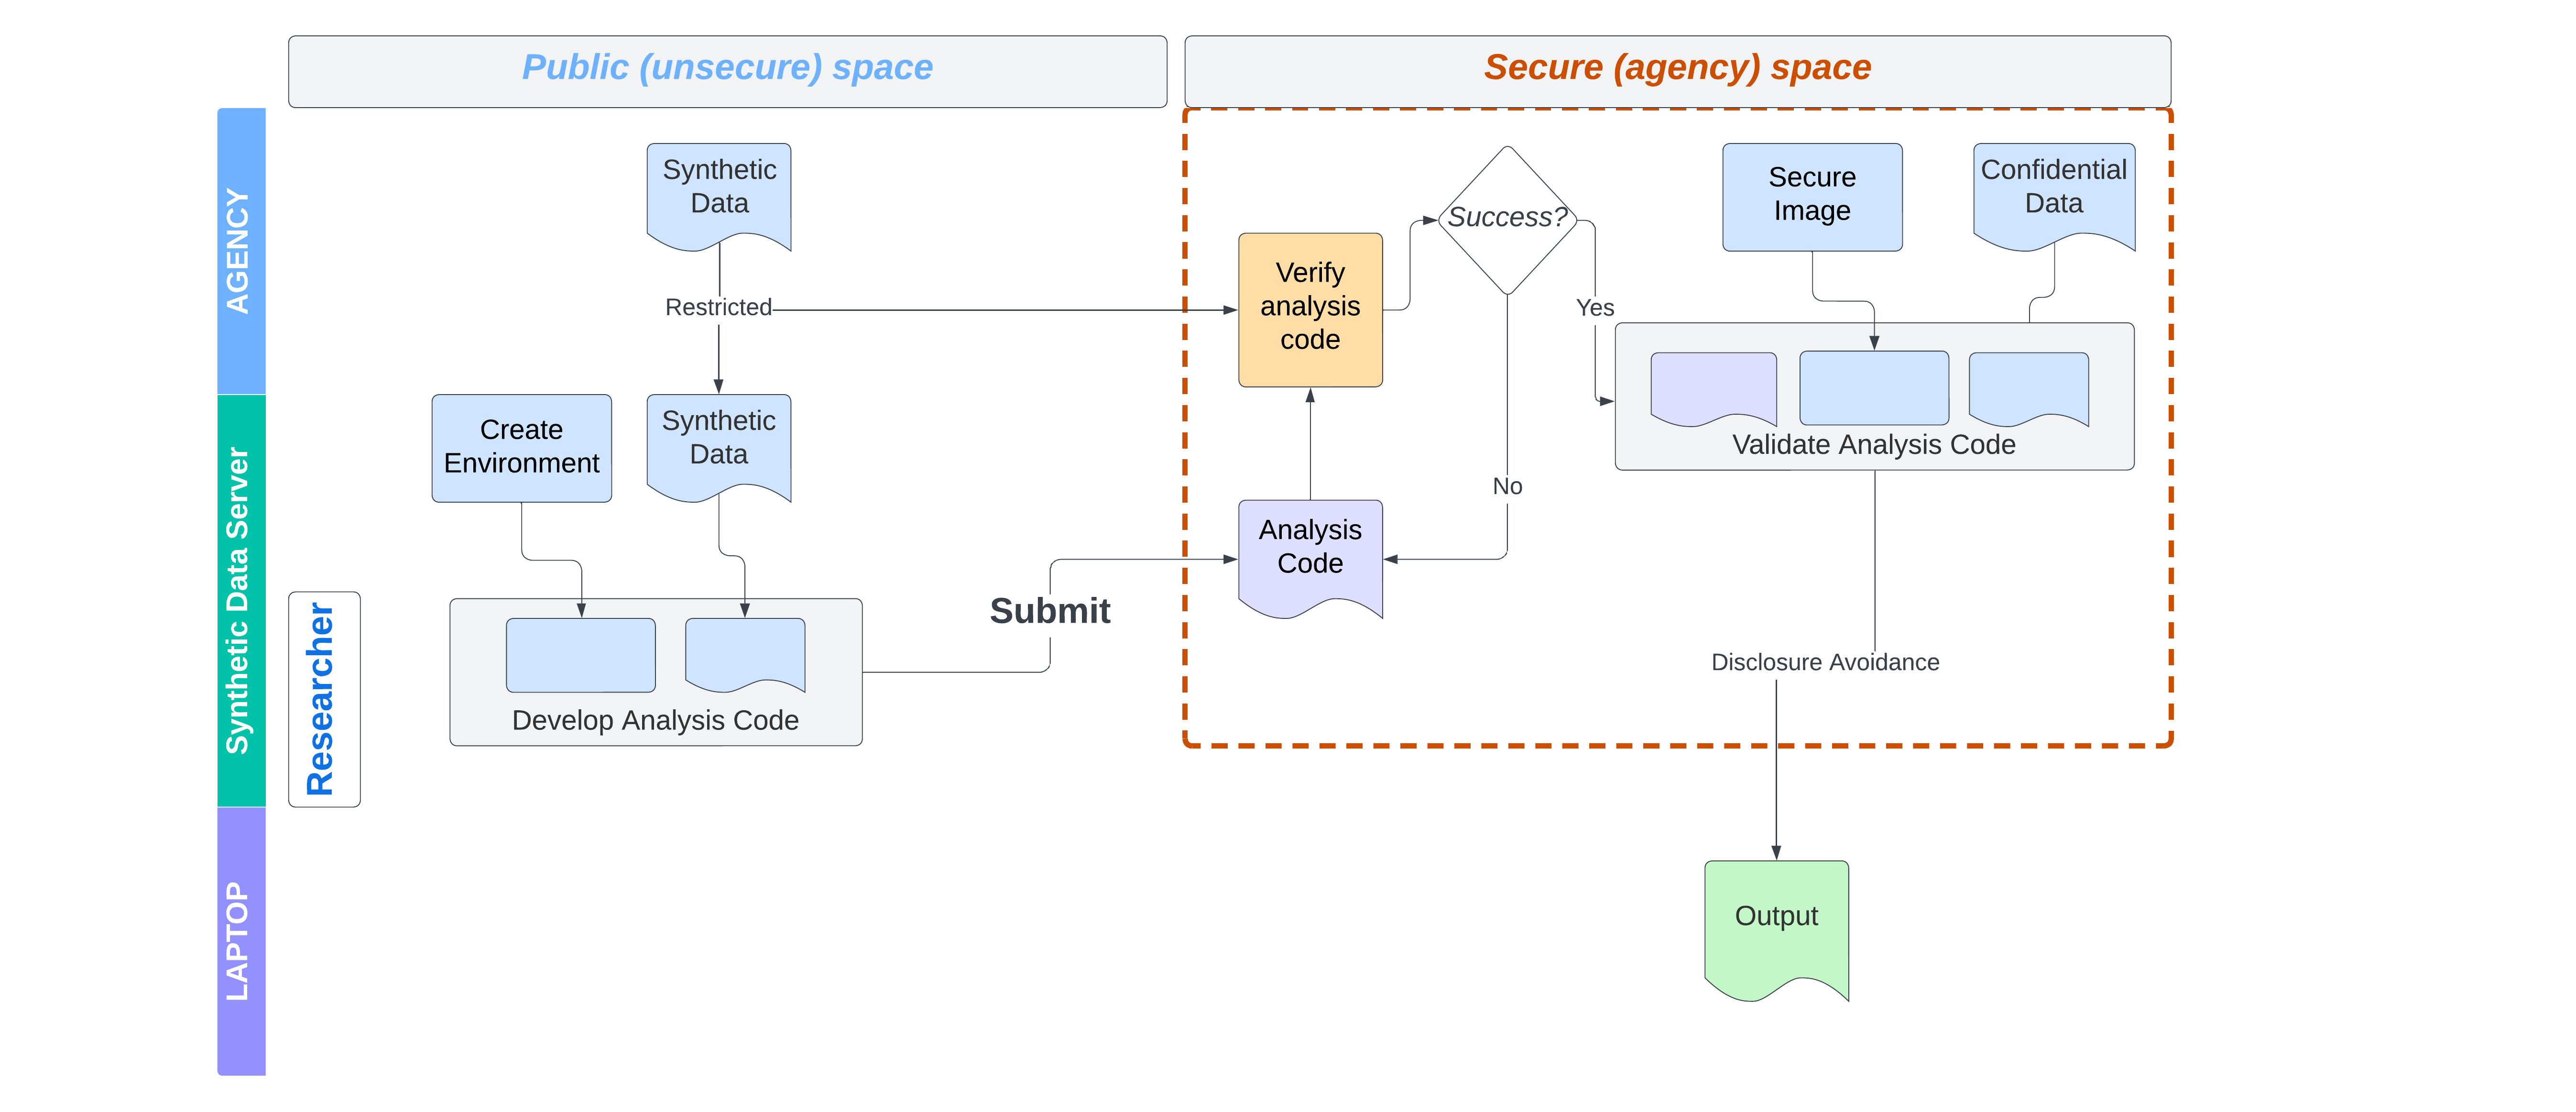
\includegraphics[width=\textwidth]{SSB Flow.png}
    % https://lucid.app/lucidchart/0d1b7aed-5a41-4f0b-9b84-adf0b7693d36/edit?view_items=VfP~hxQ8Izjc&invitationId=inv_315a286a-8880-4df0-8c68-267aefd99a79
    \caption{Process flow of validation using the Synthetic Data Server}
    \label{fig:ssb-flow}
\end{figure}


%\restoregeometry
%\newgeometry{bottom=0.5in}


\section{Lessons learned from the SDS mechanism}

Several lessons emerged from the \ac{SDS} mechanism. While many researchers used the data to write papers,
%
\footnote{All publications directly funded by the supporting NSF grant, or using the NSF-funded server, are listed at \url{https://www.zotero.org/groups/5595570/sds-nsf-1042181/library}. Some publications were prepared by NSF-funded project personnel and should not be directly included in a publication count of ``users.'' Most publications were included in this list after a bibliographic full-text search for the grant identifiers. Some researchers may not have reported the published article to the project team, or mentioned the support of the grant to the server they used in their acknowledgements.} 
%
and even organized conference sessions specifically around the use of the data,
%
\footnote{LERA session ``Data Gold! Exploiting the Rich Research Potential of Lifetime
Administrative Earnings Data Linked to the Census Bureau's
Household SIPP Survey'',  at the Allied Social Sciences 2016 Annual Meeting \citep{american_economic_association_allied_2016}. }
%
even more researchers only ``tried out'' the data. While over 100 researchers were granted access to the server to access the \ac{SSB} in the first five years of its availability (Figure~\ref{fig:growth_in_sds}), far fewer published using the \ac{SSB} data. Almost none of the published articles actually used the results produced using the synthetic data. Comparison of parameters obtained from synthetic data and from confidential data using confidence interval overlap, a measure of congruence between the synthetic data and the confidential data introduced by \citet{tas2006}, was very heterogeneous even for a given dataset across and within projects (Table~\ref{tab:overlap}).\footnote{Due to technical issues, the selection of projects is a convenience sample. The analysis was run ex-post, without the collaboration of the original authors, by injecting code into the original authors' analysis code. This often failed, especially for more complex code. The results using the confidential data were obtained by Census Bureau staff, and released to the author of this article after disclosure avoidance, several years ago.} While the results in Table~\ref{tab:overlap} do not take into account a distinction between key and nuisance parameters (simply comparing all parameters estimated in researcher-provided models), authors may have simply been very hesitant to use the parameters estimated on the synthetic data.


\begin{figure}
    \centering
    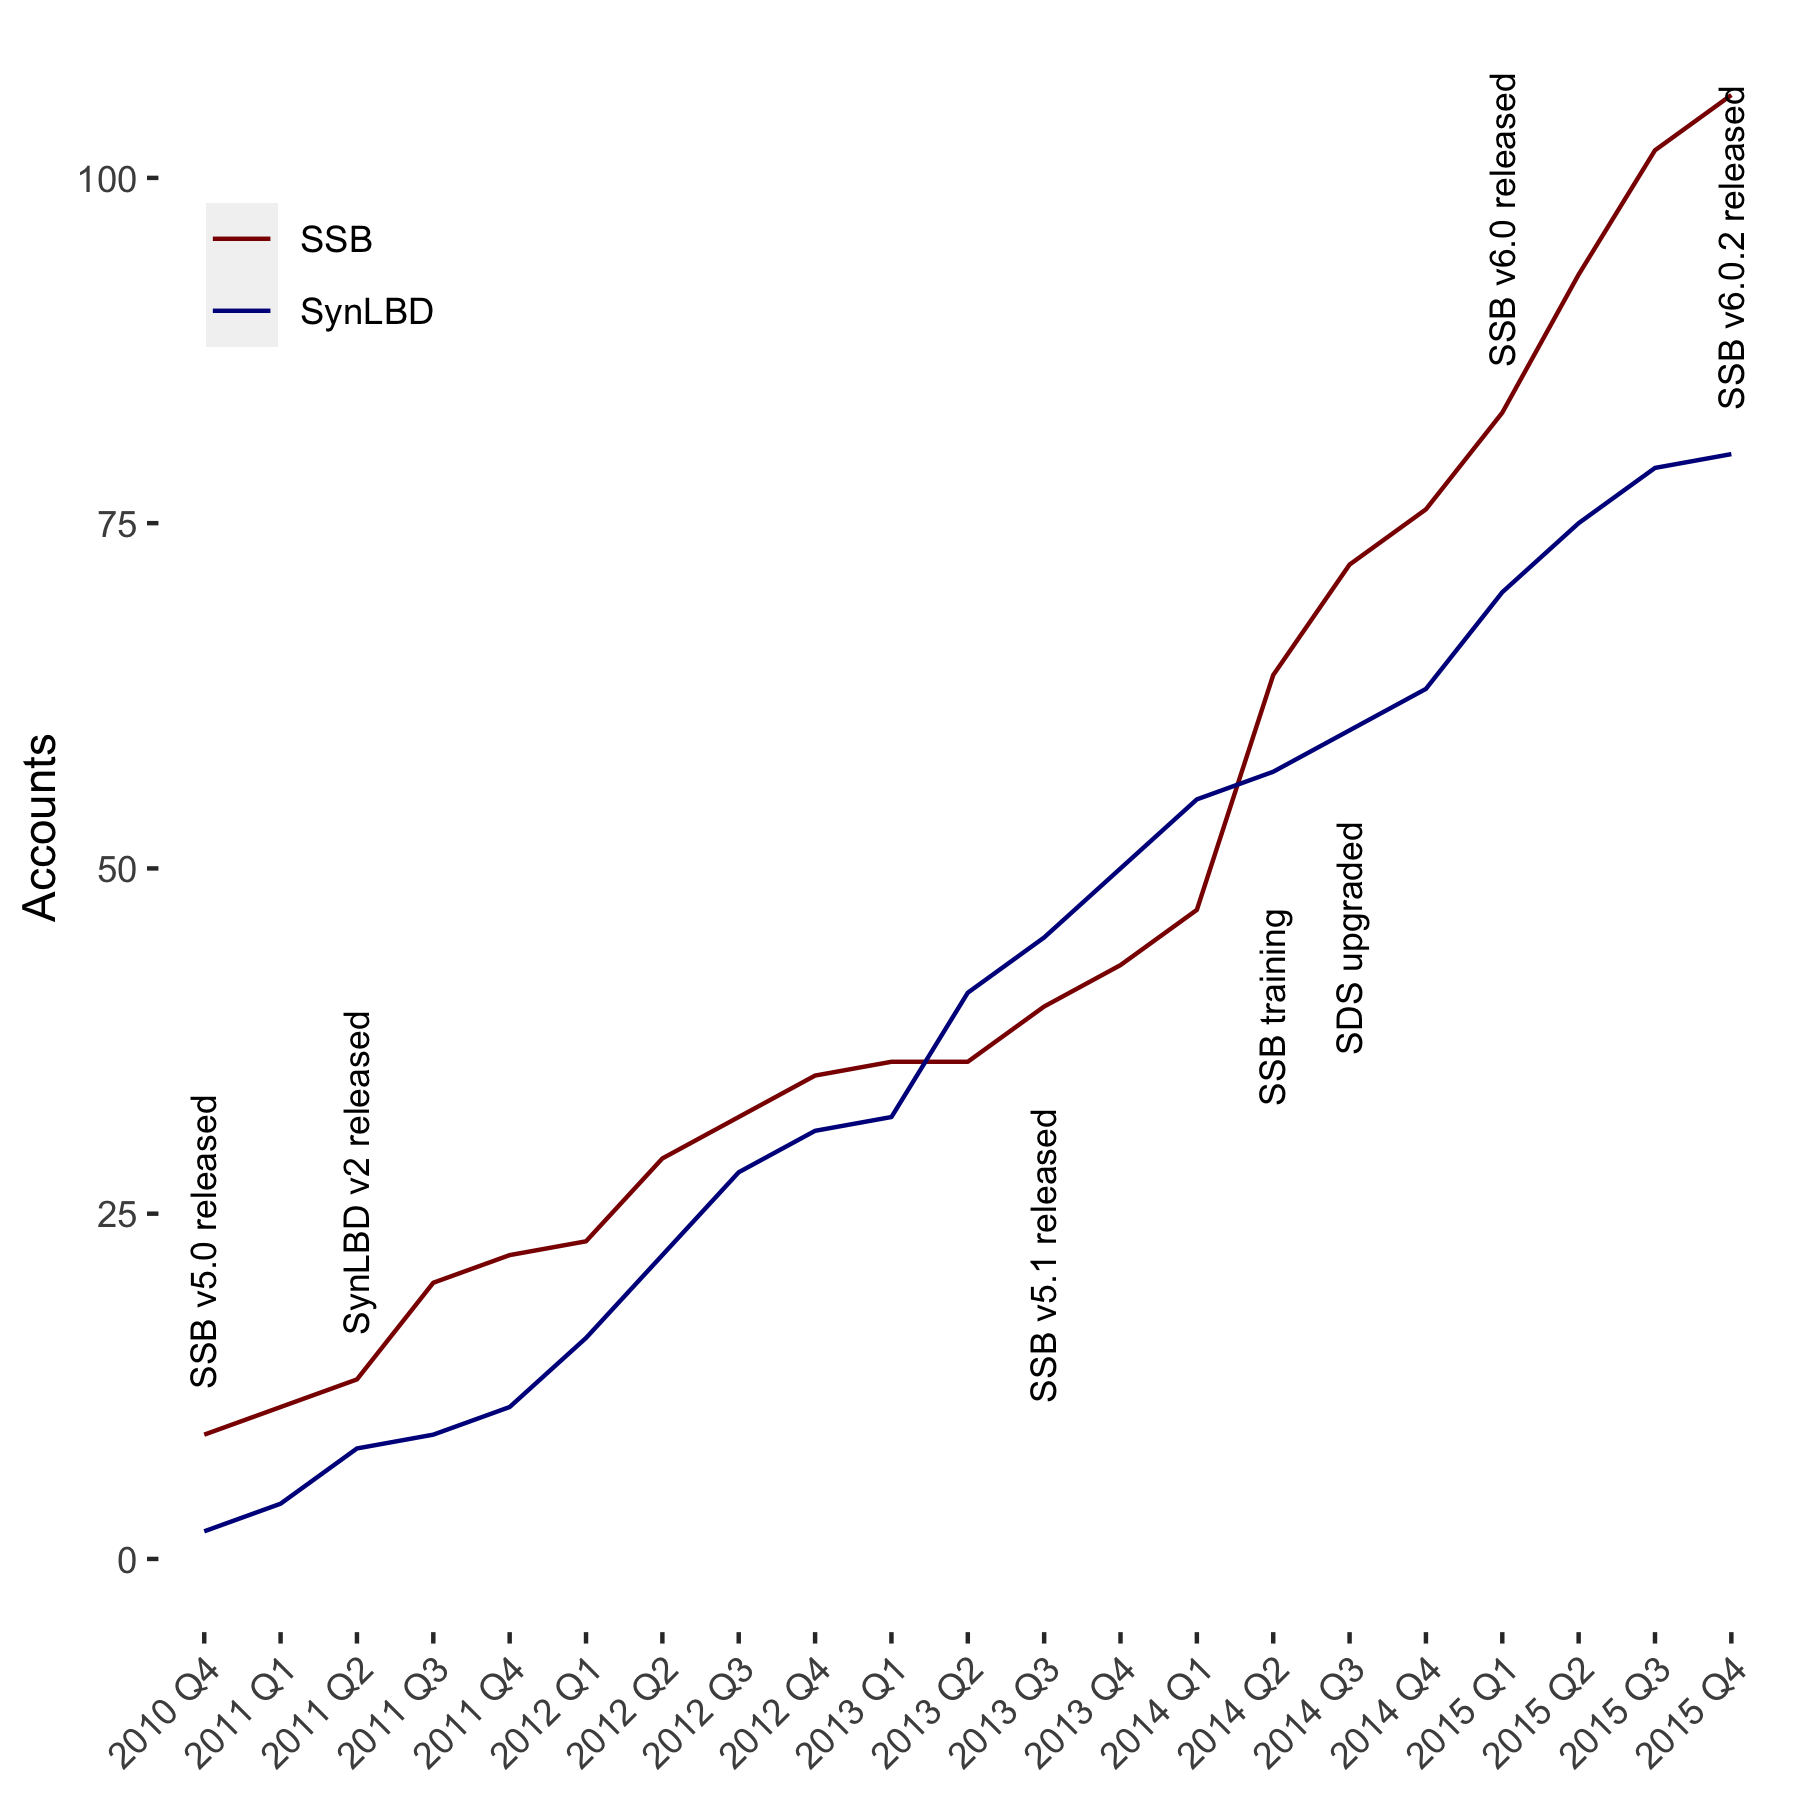
\includegraphics[width=0.8\textwidth]{accounts-2015.png}
    \caption{Computer accounts on the SDS over time}
    \label{fig:growth_in_sds}
\end{figure}

\begin{table}[]
    \centering
    \begin{threeparttable}
        % latex table generated in R 3.4.0 by xtable 1.8-2 package
% Sun Jul 16 15:50:19 2017
\begin{tabular}{llrrrrl}
  \toprule
User & Request & Mean & 75th & 90th & Max & Dataset \\ 
  \midrule
A & 1 & 0.16 & 0.25 & 0.72 & 0.89 & SynLBD \\ 
  A & 2 & 0.10 & 0.00 & 0.52 & 0.92 & SynLBD \\ 
  B & 1 & 0.87 & 1.00 & 1.00 & 1.00 & SynLBD \\ 
  C & 1 & 0.22 & 0.51 & 0.72 & 0.99 & SynLBD \\ 
  D & 1 & 0.49 & 0.79 & 0.87 & 0.98 & SSB \\ 
  E & 1 & 0.39 & 0.56 & 0.63 & 0.94 & SSB \\ 
   \bottomrule
\end{tabular}

        \caption{Distribution of Parameter-specific Confidence Interval Overlap, for selected projects}
        \label{tab:overlap}
        \begin{tablenotes}
            \footnotesize
            \item[] The table presents the distribution of overlap in parameter-specific confidence intervals \citep{tas2006} across a small number of projects (for selection, see text). The overlap is quantified as the percentage of the length of the smaller interval that is contained within the larger interval, where the pairs of intervals are defined by running the same code on synthetic and confidential data. Each row shows mean and selected percentiles from the distribution of such comparisons across all the parameters of the specific model. 
        \end{tablenotes}
    \end{threeparttable}
\end{table}
Thus, a core goal of the synthetic data --- to replace the confidential data in researchers' analyses --- was not being met, even when the synthetic data actually was a very good stand-in (note the SynLBD project B with a mean confidence interval overlap of 87\%). Nevertheless, the synthetic data were complex enough to allow for development of models without access to the confidential data, what I would call ``good enough data.''

Anecdotal evidence from both my own and Census staff's attempts to use author-provided computer code to run the analysis on the confidential data demonstrated challenges in reproducibility. Authors might hard-code intermediate findings, rather than letting the data drive the analysis, and would otherwise not fully leverage the similarity between the two computing environments. These lead to time-intensive human debugging, or multiple rounds with authors, neither of which are an efficient and satisfying process. 

More interestingly, multiple authors treated the synthetic data access as a gateway process for access to the confidential data. Knowing that the synthetic data did not contain all the features they needed for their analysis, but having to wait for permission to access the more detailed confidential data in the Federal Statistical Research Data Centers, authors used the synthetic data to prepare analyses and explore the data. Figure~\ref{fig:useRDC} shows an early analysis of the first 106 users of the \ac{SDS}, and subsequent usage of the FSRDC. 

\begin{figure}
    \centering
    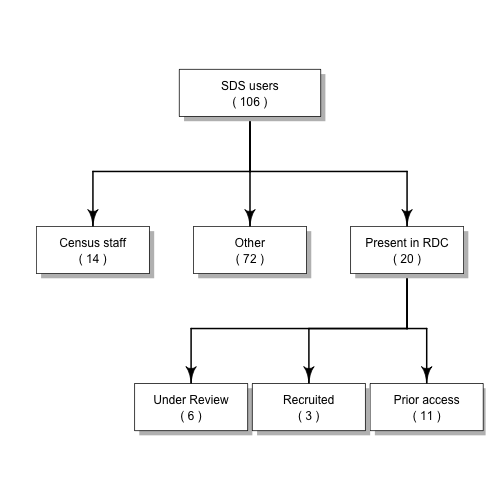
\includegraphics[width=0.5\linewidth]{useRDCgraph.png}
    \caption{SDS users and access to FSRDC}
    \label{fig:useRDC}
\end{figure}

Importantly, in the initial phase of the projects, turnaround (submission of validation request and receipt of validated and privacy-protected results) was quite fast - single-digit weeks, rather than the multi-month process of obtaining access to the FSRDC. However, the introduction of new disclosure avoidance procedures at the Census Bureau, and the lack of integration of those procedures into the validation process, greatly increased the time lag in the second half of the projects.

\section{Scaling up access to confidential data}

If data cannot be made available due to intractable disclosure avoidance issues, yet access should be broadened, what can agencies do? 
The pilot projects described earlier were not set up to scale, and yet I argue that  they demonstrated  a need for such a process. The number of researchers gaining access grew continuously (see Figure~\ref{fig:growth_in_sds}). Special sessions at conferences were organized around the data accessed in this fashion. In general, based on conversation of the author with various researchers at conferences and by email, researchers were happy with the ability to access such data without having to request a full-blown project in an FSRDC, but were somewhat frustrated by the process. 


Statistical agencies and research institutes have explored various ways to scale up access to confidential data. To cite a few examples, Statistics Canada had the Real-time Remote Access (RTRA) process, Norway has the Microdata.no system, the Bank of Portugal uses a two-stage system combining a remote desktop and validation \citep{guimaraes_reproducibility_2023}, and \citet{barrientos_providing_2018} proposed a differentially private verification server. 

Many such processes have limitations that limit their utility for researchers. The aforementioned Statistics Canada and microdata.no systems strongly limit the type of analysis that is feasible by restricting the software keywords that can be used (RTRA), by creating a structured new statistical language (microdata.no), or by limiting the types of analysis that can be run and validated \citep{barrientos_providing_2018}. Users of the Bank of Portugal's system still need to use the remote desktop system, similar to the SDS outlined before, because the data hosted there is not authorized as a full public-use product.

The issue is compounded by well-documented problems with the reproducibility of code in the social sciences. Heuristically, many of the problems with the SDS arose because the code failed to reproduce during validation, even though it was  run in a very similar environment to the development environment. Researchers in the social sciences appear to rely heavily on interactive computing, with code produced subsequently failing simple reproducibility tests.\footnote{I define ``interactive computing'' as any sequence of computational codes that must be explicitly --- through edits --- adapted to the environment it is running in, and/or does not have a streamlined workflow that can be triggered from a single file, regardless of workflow technology. Examples of workflow management ``systems'' range from \texttt{make} (1976) \citep{association_for_computing_machinery_acm_2003} to \texttt{Snakemake} \citep{molder_sustainable_2021}, to literate programming tools such as \texttt{Sweave} \citep{Leisch2002SweaveDG} and Quarto \citep{Allaire_Quarto_2024}, to simple concatenated calls to software (canonical \texttt{run.sh}). } Examples abound, and can often be gleaned from the fact that many of the reproducibility meta-studies only succeed in reproducing a small number of studies due to limitations in personnel time.%
\footnote{\citet{stockemer_data_2018} note ``lack of organization in code and data presentation was the main reason that we were unable to replicate some results'' in political science articles. \citet{StoddenPNAS2018} notes that only 32\% of packages in Science required only minor or no effort to reproduce, though some of the reasons listed are unavoidable (GPU setup, custom hardware) and not related to workflow issues. For the economics journal studied in \citet{herbert_reproduce_2024}, only 24\% required no change to the code in order to be able to run, even when the ultimate results was full reproducibility.}
%
In a sample of over 8,000 replication packages associated with high-profile economics articles, only 30\% had some sort of master script.\footnote{Code run in November 2023, searching for any filename that contained the strings `main' or `master', the most common name used for control code in economics. I am not aware of a similarly comprehensive collection for other social sciences.} This is also my impression from our own efforts at the LDI Replication Lab supporting the AEA Data and Code Availability Policy, though we no longer make a systematic effort to categorize this.  In part to cater to this need, remote-access or local secure access in the form of physical or virtual secure data enclaves are still the dominant - but expensive - way to access confidential data. The dominant method of access thus forces researchers to choose between lower quality data in an environment that corresponds to their preferred computing method, and higher quality confidential data in environments that are expensive for researchers, data providers, or both.

\section{Desiderata}
\label{sec:desiderata}

Drawing on the experience from the SDS pilot projects and other remote access methods used in the past, as well as looking at newer technologies that have emerged in the last decade, I suggest that a new, scalable mechanism to provide access to confidential data should have the following desirable characteristics:

\begin{enumerate}[label={[D\arabic*]}]
    \item the mechanism must support arbitrary modeling approaches and ideally a large number of programming languages
    \item the mechanism must allow for development of models by researchers that are close to their ``normal'' method of developing models
    \item the mechanism must be low-cost for the data provider, scaling at best sub-linearly with the number of users of those datasets
    \item the mechanism must be low-cost for the data user, imposing at best marginal costs on their existing research infrastructure (software, computers)
    \item the privacy-protected data provided as part of such mechanisms must be good enough to allow for complex modeling
    \item validation, if necessary, must be fast - on the order of hours
\end{enumerate}

Note that public-use data, as historically provided by statistical agencies, satisfies all of these criteria, except for the last one. Should statistical agencies actually offer validation even for such public use data, as \citet{reiter_verification_2009} have argued? Traditionally, they do not, and leave it up to individual researchers to ``self-validate'' by requesting access to confidential data in a time-consuming fashion.\footnote{See \citet{armour_using_2016} for one example of such a project, affecting the widely-used Current Population Survey.}

\section{A Proposal using Containers}
\label{sec:proposal}
I demonstrate a simple scenario that satisfies most of the desiderata,  using containers.  Containers can easily be validated for reproducibility before they are then forwarded to the confidential computing environment. Once determined to be reproducible, they can then extend the analysis to use confidential data, and enable a wide spectrum of plug-in disclosure avoidance measures as well. Crucially, all validation of reproducibility can be performed prior to validation using the confidential data, on open, possibly commercial platforms. Only once reproducibility is confirmed is the same analysis model ported to the confidential data. The concept here is similar in principle to a ``Common Task Framework'' \citep{liberman_obituary_2010,liberman_reproducible_2014,liu_successes_2019}, but applied to the access problem around confidential data, not to a validation or holdout dataset \citep{liu_successes_2019,donoho_data_2024}.\footnote{I thank an anonymous referee for having pointed out this analogy.}  

The use of cloud providers removes the requirement for users of the synthetic data to install anything locally. The open-source nature of the container technology, on the other hand, allows users to do so, when they want to, or when they have to. The use of containers enforces reproducibility out-of-box when using synthetic data. Furthermore, containers enable scalability. 

Finally, the combination of assured reproducibility and easily scalable computation allow for streamlined validation against the confidential data, which is in essence a replication of the analysis on the synthetic data. The streamlining, in turn, allows for low-cost rapid turnaround, quickly providing feedback and possibly results to researchers who otherwise do not have access to the confidential data. And by doing so quickly, the need to have complex and fully analytically valid synthetic data in the first place may no longer be binding. This, in turn, allows data providers to reduce the amount of time and effort devoted to developing complex synthetic data, instead focusing on creating plausibly complex, possibly custom-generated, low fidelity synthetic data, at low or no cost to disclosure avoidance budgets.

The use of containers in this way is novel as a systematic way to provide scalable, potentially high-throughput validation, and differs in usage from previous methods, such as the Cornell Synthetic Data Server. Containers have been used in a small number of well-published instances in the economics literature for precisely this kind of purpose, and are well-understood in the computer science and statistics community \citep{boettiger_introduction_2015,moreau_containers_2023}. Nevertheless, acceptance in the social science community  is not great, so far. In the same 8,000 replication packages in economics mentioned earlier, only 0.13\% had used containers. While hard evidence in other social sciences is difficult to come by, none of the studies that analyzed reproducibility in the various social science disciplines mention the use of containers as the primary tool to ensure reproducibility in any of the packages they have analyzed.

\subsection{Details}


Reproducibility is important for synthetic data products when there
is a validation or verification process involved. In such a setting, data users will first use the synthetic
data to build and test their code for a desired analysis. Once the user is satisfied with the code used to
perform their analysis, they can request validation or verification, and their code will be run by the data provider on the confidential data. Output from the analysis on the confidential data will then have to satisfy the data provider's disclosure avoidance procedures before it can be released to the user. In the case of validation, the results from the second run on confidential data are released to the user, possibly confidentialized \citep{u.s.censusbureauSIPPSyntheticBeta2015b}. In the case of a verification server, the user only receives a (non-disclosive) message indicating whether her results from the first run can be considered to be inferentially valid or not \citep{barrientos_providing_2018}.

One problem that can arise when maintaining a validation process is that the 
computing environment on the data user's end does not exactly match the computing environment for
the internal validation. This can lead to validation attempts that fail to run correctly or at all, which
increases the wait time for data users and the staff time involved in performing the validation at the data provider. 
In order for this process to run smoothly, the data user's code needs to be reproducible.  This ensures that the user's code can be easily transferred and
run on the confidential data. This can be achieved by using a ``container.'' A container collects all of the
necessary libraries, dependencies, and code needed to run an analysis in a single
package. This container can then be downloaded to any machine and used with the local system to run
the application. Crucially, container systems usually have the capability to either rebuild containers in a trusted environment, or to provide to users pre-configured secure containers that are also authorized to run in the secure area hosting the confidential data. In most cases, the core container itself does not need to be transferred, only a comprehensive, easily parsable recipe to build such a container from known sources, and the user's model-specific code. Both the recipe (called a `Dockerfile') and the user-provided model code, are plain-text, and adhere to known language specifications, which allows for easier security vetting of the code.

\section{A detailed use case when using synthetic data}
\label{sec:usecase}

In this section, we walk through the process for a specific use case. The Census Bureau, data owner (custodian) of the confidential SIPP file merged with administrative data known as the SIPP Gold Standard file, makes a synthetic version of the Gold Standard file available as the \ac{SSB} \citep{Benedettoetal_2013}. The container host in the public domain in this case is Codeocean, which provides cloud-based access to Docker-based containers (called ``compute capsules``).\footnote{There are many commercial providers able to run Docker containers.} We use the example of Codeocean here, because they provide a relatively user-friendly interface for development of code, while retaining the requirement to have a hands-off, non-interactive run as a pre-requisite for publication.  Crucially, Codeocean provides access to Stata and MATLAB compute capsules, covering 95\% of economists' software needs. Users log in via a simple web browser, with no install required. A Codeocean capsule can, however, also be used by researchers on their own workstation, as long as they have Docker installed (or a compatible container runtime) and have a Stata or MATLAB license. Because of the standards-based approach, it is also straightforward to exchange the configured Codeocean-generated ``base image'' for a security-vetted base image within the confidential environment, something we return to later.%
%
\footnote{The basic functionality can be achieved on any container system. Other services in this space include  or have included {Wholetale} \citep{brinckman_computing_2018,chard_toward_2020}, \href{https://www.onyxia.sh/}{Onyxia}, and many others. An earlier version of this article mentioned Gigantum, and linked to the website of Wholetale. As is not unusual in this space, Gigantum no longer functions as a company, and Wholetale, as an academic, externally funded pilot project, is no longer available. However, with the right setup, the open-source specification of most current container technology do not depend on any single provider.} 
%
Finally, users who wish to not use such services can also typically provide their own setup for the synthetic data component, at very little additional cost or effort. Many university computing system provide some support on their high-performance computing clusters. For data providers, the tools used (containers) are widely used by numerous cloud providers, are transparent in how they are built, and allow for in-depth security scanning while retaining much of the flexibility that researchers and IT providers seek.

In this configuration, the Census Bureau could allow Codeocean to house both the synthetic dataset as well as
setup and configuration code that will assist the data user in creating code that is reproducible. The data
user can then build on the setup and configuration code provided by the Census Bureau to perform their
desired analysis. To perform the analysis on the synthetic data, users may either run the code directly on
Codeocean by paying for access to computing resources\footnote{At the time of writing, Codeocean  provides a limited amount of storage space and computing time for free to academic users.} or they may download the compute capsule, including the synthetic data, to their local
machine and use their own computing resources. When the user requests validation, they provide or point to the compute capsule (containing code and any external data). The Census Bureau can then  securely rebuild the container (if necessary), and make minimal (automated) changes to execute the analysis in a
secure computing environment with the confidential data. By ensuring that everything can
run within the Codeocean compute capsule using the synthetic data, it also makes it very likely that everything can
be run within the associated compute capsule's container using the confidential data, even when the confidential data is not housed on Codeocean or any publicly accessible service.
In addition to providing a location for the Census Bureau and data users to share access to the synthetic
dataset and code, this mechanism also greatly increases the probability that the analysis will run correctly for both the data user and on the
confidential data. 



\subsection{Development of code on open compute servers using synthetic data}

Basic structure of Codeocean's existing validation process\footnote{See \url{https://help.Codeocean.com/getting-started/uploading-code-and-data/paths}} imposes a strict separation between code, immutable data, and reproducible results:\footnote{While there are various standards on the publication of research code, this is not meant to be yet another one. This is purely a requirement of the validation process, as implemented by this provider. The data custodian would need to define what their required structure is, which may or may not adhere to a specific code publication standard.}

\begin{itemize}
    \item all code is under \texttt{/code}
    \item all data are under \texttt{/data}
    \item all outputs MUST be written to \texttt{/results}, otherwise they are lost.
\end{itemize}

Outputs are regenerated at each run, and the history of such runs can be found (for the developing user) in the right pane. When the user, at the end of the development process, requests publication of the compute capsule, only the last run is published, together with code and data.

To facilitate this file organization for the user,  template code, provided by the agency, can include a configuration file, which applies best programming practices by defining  global variables for file paths that are used elsewhere in the code, and which can be modified by runtime environment variables. For instance, the default file path to the data location may be supplied by the operating system in the confidential environment, switching where any user code will look for data. On the open compute server, the same configuration file would seamlessly point to the synthetic data. The template code also instantiates logfiles, which are also written to \texttt{/results}, which allow for verification of what happens during runtime.


%## The use of external packages

Stata, R, and many other programming languages use external packages of code (libraries) to augment native capabilities. Initially, these need to be installed over the internet. However, there are various ways to address the issue at subsequent installations: (1) Packages can always be re-installed from source at runtime; (2) packages can be installed by a programming-language specific install script at (first) runtime, and stored locally; and (3) packages can be incorporated into the container image itself (package installation is included in the recipe.

Codeocean has the ability to do the third method, via a ``post-install'' script that is run when the environment is setup (the project-specific container image is built). This embeds any such libraries into the container image, rendering subsequent internet access unnecessary for the software to run. However, this particular environment also supports the two other methods. This could lead to failure in a confidential computing environment that does not allow for internet access, and will need to be specified to users.\footnote{The use of software-specific environments in R, Python, Julia, and also Stata might also render subsequent internet access unnecessary when using the second method, but also requires software-specific checks to verify whether this is actually done correctly.}

I note that while hosted on Codeocean, the same image, once built, is re-used, and packages installed using the third method are not re-installed. However, when exporting a capsule, only the build script is exported, and a replicator would need to rebuild the container, thereby also re-installing any packages. This can lead to version discrepancies when packages cannot be pinned to a particular version (as is the case with Stata). 

\subsection{Validating reproducibility}

The Codeocean interface signals to researchers the successful completion  of the controller script (called \texttt{run}) in the right pane of the user interface. To the custodian of the confidential data, this indicates that the code is verified to execute without error on the synthetic data. The results produced by this specific run of the controller script, and not any previous interactive run, are the results provided in the ``results'' pane.  It is important to highlight here that the Codeocean implementation preserves no outputs from prior runs in the ``results'' pane and folder, only from the latest run. It is thus not possible for researchers to create output in a prior run, then to comment out code that would then not be reproduced in a subsequent run in the confidential environment. Only fully automated complete runs produce all the expected output. This is important for scalability and efficiency, as it reduces the need for extensive debugging, on the researcher side, and allows for rapid assessment of basic reproducibility by the data custodian. 



%%%%%%%%%%%%%%%%%%%%   EXAMPLE

\subsection{Estimating Economic Returns to Education in the SIPP}

I now provide a concrete, albeit only theoretically possible, example. In this example, code to estimate  a standard Mincer earnings equation \citep{mincer_schooling_1984,heckman_fifty_2003} on the SIPP Synthetic Beta data \citep{u.s.censusbureauSIPPSyntheticBeta2015b}. The code as provided here is in Stata, the dominant statistical programming language for economists \citep{10.1257/pandp.110.764}, though it could just as easily have been produced in any other statistical programming language.\footnote{Note that the current \ac{SSB} access mechanism \citep{u.s.censusbureauSIPPSyntheticBeta2015b} requires the use of Stata or SAS.} The code is split into 4 pieces, tied together by a (system-defined) controller script. Listing~\ref{code:stata-mincer} provides the code for the main analysis in this example. The fully worked out example can be found at \href{https://github.com/larsvilhuber/ssb-demo/releases/tag/v20250403}{Github}.


\lstinputlisting[language=stata,caption={Example Analysis Code in Stata},breaklines=true,label={code:stata-mincer}]{02_mincer.txt}

% ### Script

% The script [run](run) ties all Stata programs together. An alternative would be to have both a generic run, plus a master Stata do file. Both options work.

% ### Stata programs

% - [config.do](config.do) creates various global variables, and initializes a per-program log file, which will show up in `/results`.
% - [00_setup.do](00_setup.do) initializes the code setup for each run. 
%   - It could also install Stata packages from SSC (see discussion above).
% - [01_stats.do](01_stats.do) computes a few simple descriptive stats. Only log output is generated, but this could generate a summary stats table (``Table 1``) of a paper.
% - [02_mincer.do](02_mincer.do) does data prep and runs a Mincer regression. Output is generated through `esttab`, and stored in `/results/mincer_results.csv`.



\subsection{Dockerfile}

The environment is specified through a Dockerfile. The Dockerfile in this case specifies the use of a Codeocean-specific pre-built Stata container as the source, injects a valid Stata license, and handles installation of any Stata packages (the third method, mentioned earlier). Listing~\ref{code:dockerfile1} shows the complete recipe, illustrating the simplicity of this approach. 

\lstinputlisting[language=docker,caption={Example Dockerfile},breaklines=true,label={code:dockerfile1}]{dockerfile.1.txt}

\subsection{Executing code on public (synthetic) data using commercial infrastructure}

Once the user has developed all the code, they execute a ``reproducible run'' on Codeocean. This ensures that all code executes without error (note that it does *not* ensure that all necessary code has run - code can be commented out or be non-functional). This particular example, when run on Codeocean infrastructure in 2021, takes about 4 minutes to execute.\footnote{Unfortunately, at the time of this writing, Codeocean does not have the ability to remove data from a published compute capsule, and the Census Bureau's current license for the SSB data does not allow to publish the synthetic data. Thus, we cannot actually point to a public instance of the compute capsule.}

\subsection{Executing code on public (synthetic) data using private or academic infrastructure}

Alternatively, the user can export the entire capsule (including data), rebuild the image locally, and execute on their local infrastructure, using an unmodified Dockerfile. Listing~\ref{code:build} illustrates this process when run on an appropriately configured personal computer.\footnote{Note that the image thus created should not be publicly posted, as it contains a valid Stata license file. See \href{https://github.com/AEADataEditor/docker-stata} for a discussion on how to build Docker images that can be distributed openly, while mounting a license only at run-time.}

\lstinputlisting[language=bash,basicstyle=\footnotesize\color{NavyBlue}\ttfamily,caption={Building the container},float,label={code:build}]{docker-build.txt}
%

\noindent Running the actual code on the user's personal computer is then very straightforward (Listing~\ref{code:run}).


\lstinputlisting[language=bash,basicstyle=\footnotesize\color{NavyBlue}\ttfamily,,caption={Running the container},label={code:run}]{docker-run.txt}



\subsection{Submitting code to the agency}

Once the user is satisfied, they can submit their code to the Census Bureau, much as they are requested to do at present \citep{u.s.censusbureauSIPPSyntheticBeta2015b}. Notably, they would not submit the Docker \textbf{image} built in the previous step, or provided by Codeocean, only, if modified, the Dockerfile (see Listing~\ref{code:submit}).

\begin{lstlisting}[language=bash, caption=Submitted files,basicstyle=\footnotesize\color{NavyBlue}\ttfamily,label={code:submit}]]
./code/00_setup.do
./code/01_stats.do
./code/02_mincer.do
./code/LICENSE
./code/README.md
./code/config.do
./code/run
./environment/Dockerfile
\end{lstlisting}


The agency can do all the usual checks on the (plaintext) statistical code, and can verify if any modified Dockerfile might cause any issues. This can be done using simple tools like \texttt{diff} (Figure~\ref{fig:docker-diff}).

\begin{figure}[hbt]
    \centering
    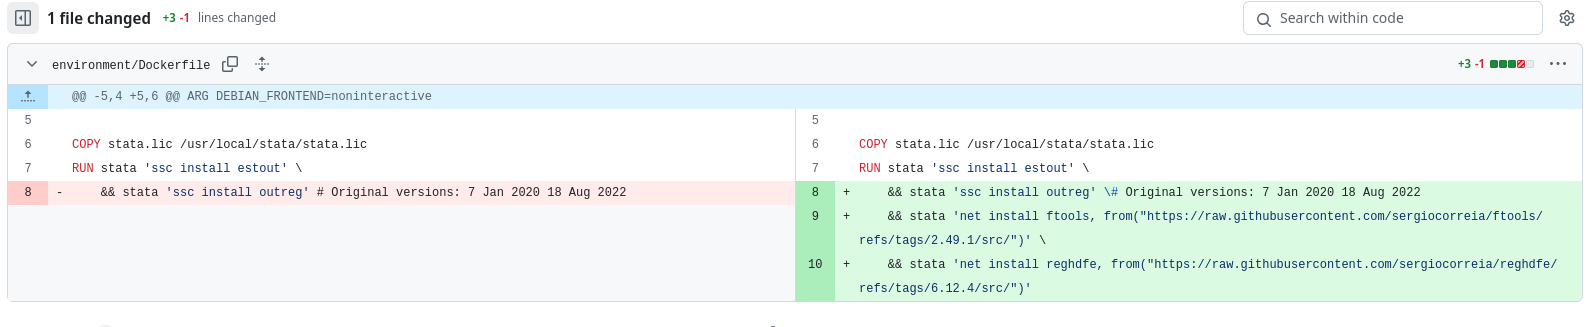
\includegraphics[width=1\linewidth]{diff-wide-dockerfile.png}
    \caption{Checking modifications to user-provided container recipe}
    \label{fig:docker-diff}
\end{figure}

Importantly, all such content-based checks should be clearly identified to the users, and could be  implemented during an upload process, so that efficient and rapid feedback is given to users. 

\subsection{Validating researcher-provided code}

While Codeocean or other providers may confirm that the code runs reproducibly, there may be situations where the data custodians wants to separately validate reproducibility. They may have doubts, because some of the code is commented out, or any other indicator that would warrant further inspection. One possible reason is that the code was not actually validated by a commercial provider. The agency  can then also run the container again, in an unsecure environment, using the synthetic data, possibly fully automated as part of the submission system. Nothing needs to pass into the secure environment for this to happen.\footnote{How to do this as part of open infrastructure is demonstrated at \url{https://github.com/labordynamicsinstitute/continuous-integration-stata}.} 





\subsection{Porting to confidential compute server}

In order to conduct a validation exercise, the code needs to be re-executed in the secure data environment. If the user used Codeocean and transmitted the capsule identifier, the compute capsule can be exported (via ``Capsule -> Export``) or more likely, pulled via an API. If the user submitted code to a web interface (Listing~\ref{code:submit}), then the agency already has the code.\footnote{In both cases, pulling the code via `git' might also be an option.} Since exporting the package is done here by the data owner, exporting the (synthetic) data is not necessary, making for a light package. 

\subsection{Dynamic code provided by data custodian}

As configured in the present example, the code requires only minor modifications to work on confidential data. The data custodian can provide a `config.do`  that can handle switching from synthetic to confidential for specific code pieces (Listing~\ref{code:config.do}).\footnote{\texttt{sed -i 's/confidential no/confidential yes/' config.do} would do the trick.}

\lstinputlisting[language=stata,breaklines=true,caption={A dynamic configuration file},label={code:config.do}]{config.do}

Alternate methods exist as well. For instance, one could test for presence of ```config-confidential.do`'' and include it if present, overriding any parameters in the main `config.do`, or rely on environment variables. Equivalent methods exist in all programming languages.

\subsection{Modifying the container base image}

The Codeocean capsule uses a Codeocean-specific prebuilt container used to execute the code (in the case of this capsule, \url{registry.codeocean.com/codeocean/stata:16.0-ubuntu18.04}). This image will need to be replaced with a container that satisfies the data owner's security requirements, while maintaining full compatibility with the needs of the environment. Because this example uses Stata, which behaves fairly uniformly across various Linux installs, the particular version of the Linux base image is likely not important.   Alternatively, the validation exercise can be coordinated with the provider, and the provider can offer a generic security-vetted image that is verified to be functionally equivalent to the image used in the secure environment. Finally, the Docker file underlying the \texttt{stata:16.0-ubuntu18.04} image, which builds the container from scratch, can be used to rebuild a container within the secure environment.\footnote{\href{github.com/AEADataEditor/docker-stata/releases/tag/stata16-2021-06-09}{https://github.com/AEADataEditor/docker-stata/releases/tag/stata16-2021-06-09} for an example.} At scale, this would simply use a similar, security-vetted, pre-built container available within the secure agency environment, e.g., \url{registry.census.gov/codeocean/stata:16.0-ubuntu18.04-secure}.\footnote{This is a fake URL, no such registry currently exists}

The key feature here is that no binary code needs to be transferred into the secure environment, eliminating a substantial security risk. Only the user-provided Stata code is needed for the validation, and a limited modification of the Dockerfile. The former is already being transferred to the agency for validation activities, and at a much larger scale within secure environments such as the \acp{FSRDC}. Only the transfer of the Dockerfile is new. Since execution is in a controlled environment, and can be trivially separated from other sensitive areas (code cannot ``break out'' of the container), security is substantially enhanced. The execution environment is completely known to the IT personnel of the data provider. Because all code should be basic ASCII or UTF-8 text, malware or more enhanced code scanners should have no problem verifying the safety of the code. I discuss additional security considerations later.

\subsection{Replacing the input data}

Finally, the synthetic input data available in the public-facing environment needs to be replaced by confidential data. In the Stata code, this is already handled, as outlined above. In order to make this actionable, the Docker image can be executed in a particular fashion, provisioning the container with confidential data. Consider a directory with confidential SSB data (\texttt{\$CONFDATA}) that looks like this:

\begin{lstlisting}[language=bash]
/path/to/confidential/data:
  - ssb_v7_0_confidential1.dta
  - ssb_v7_0_confidential2.dta
  - ssb_v7_0_confidential3.dta
  - ssb_v7_0_confidential4.dta
  - ssb_v7_1_confidential1.dta
  ...
  - config-confidential.do   
\end{lstlisting}

To run the provided capsule on confidential data, the confidential data directory is  bind-mounted into the container, as is the configuration file for the confidential data (\texttt{config-confidential.do}). Results are stored in a request-specific output area (here referenced by \texttt{\$REQUEST}). Results are written into a \url{results-confidential} directory, denoting that they have not yet been vetted by data provider's disclosure avoidance procedures. All of this is under control of data provider. Listing~\ref{code:run-conf} shows how this would be implemented as a  modification of Listing~\ref{code:run}, although it is more likely to be run within an automated environment. 



\lstinputlisting[language=bash,
           basicstyle=\footnotesize\color{NavyBlue}\ttfamily,
           caption={Running the container with confidential data},
           label={code:run-conf},
           emph={ 2, 4, 6},
           emphstyle=\colorbox{yellow}
           ]{docker-run-conf.txt}


\noindent However, it should be noted that the container does not have to be used for the validation. If the internal computing environment is faithfully reproduced by the container environment, then simply running the code, in combination with the \texttt{config-confidential.do}, may be sufficient. Thus, while containers are key to providing a user-facing environment, they are not a necessary condition for use within the existing secure computing environment.

\subsection{Sending results back to user: output vetting}

Once results have been generated, the usual disclosure avoidance workflow at the data provider is triggered. This might entail post-processing of the results, generation of additional supporting statistics (though these should generally be included in the processing), and finally, provision of the results to users.\footnote{I call this ``usual'', since I make no assumptions about changes to existing laws on data confidentiality that an agency is subject to. In order to be implementable, all data access, whether directly or via this new mechanism, must still be compliant with the laws that the agency is subject to, though some re-interpretation of what are permissible uses may be a separate channel to speed up access.}

\begin{figure}
    \centering
    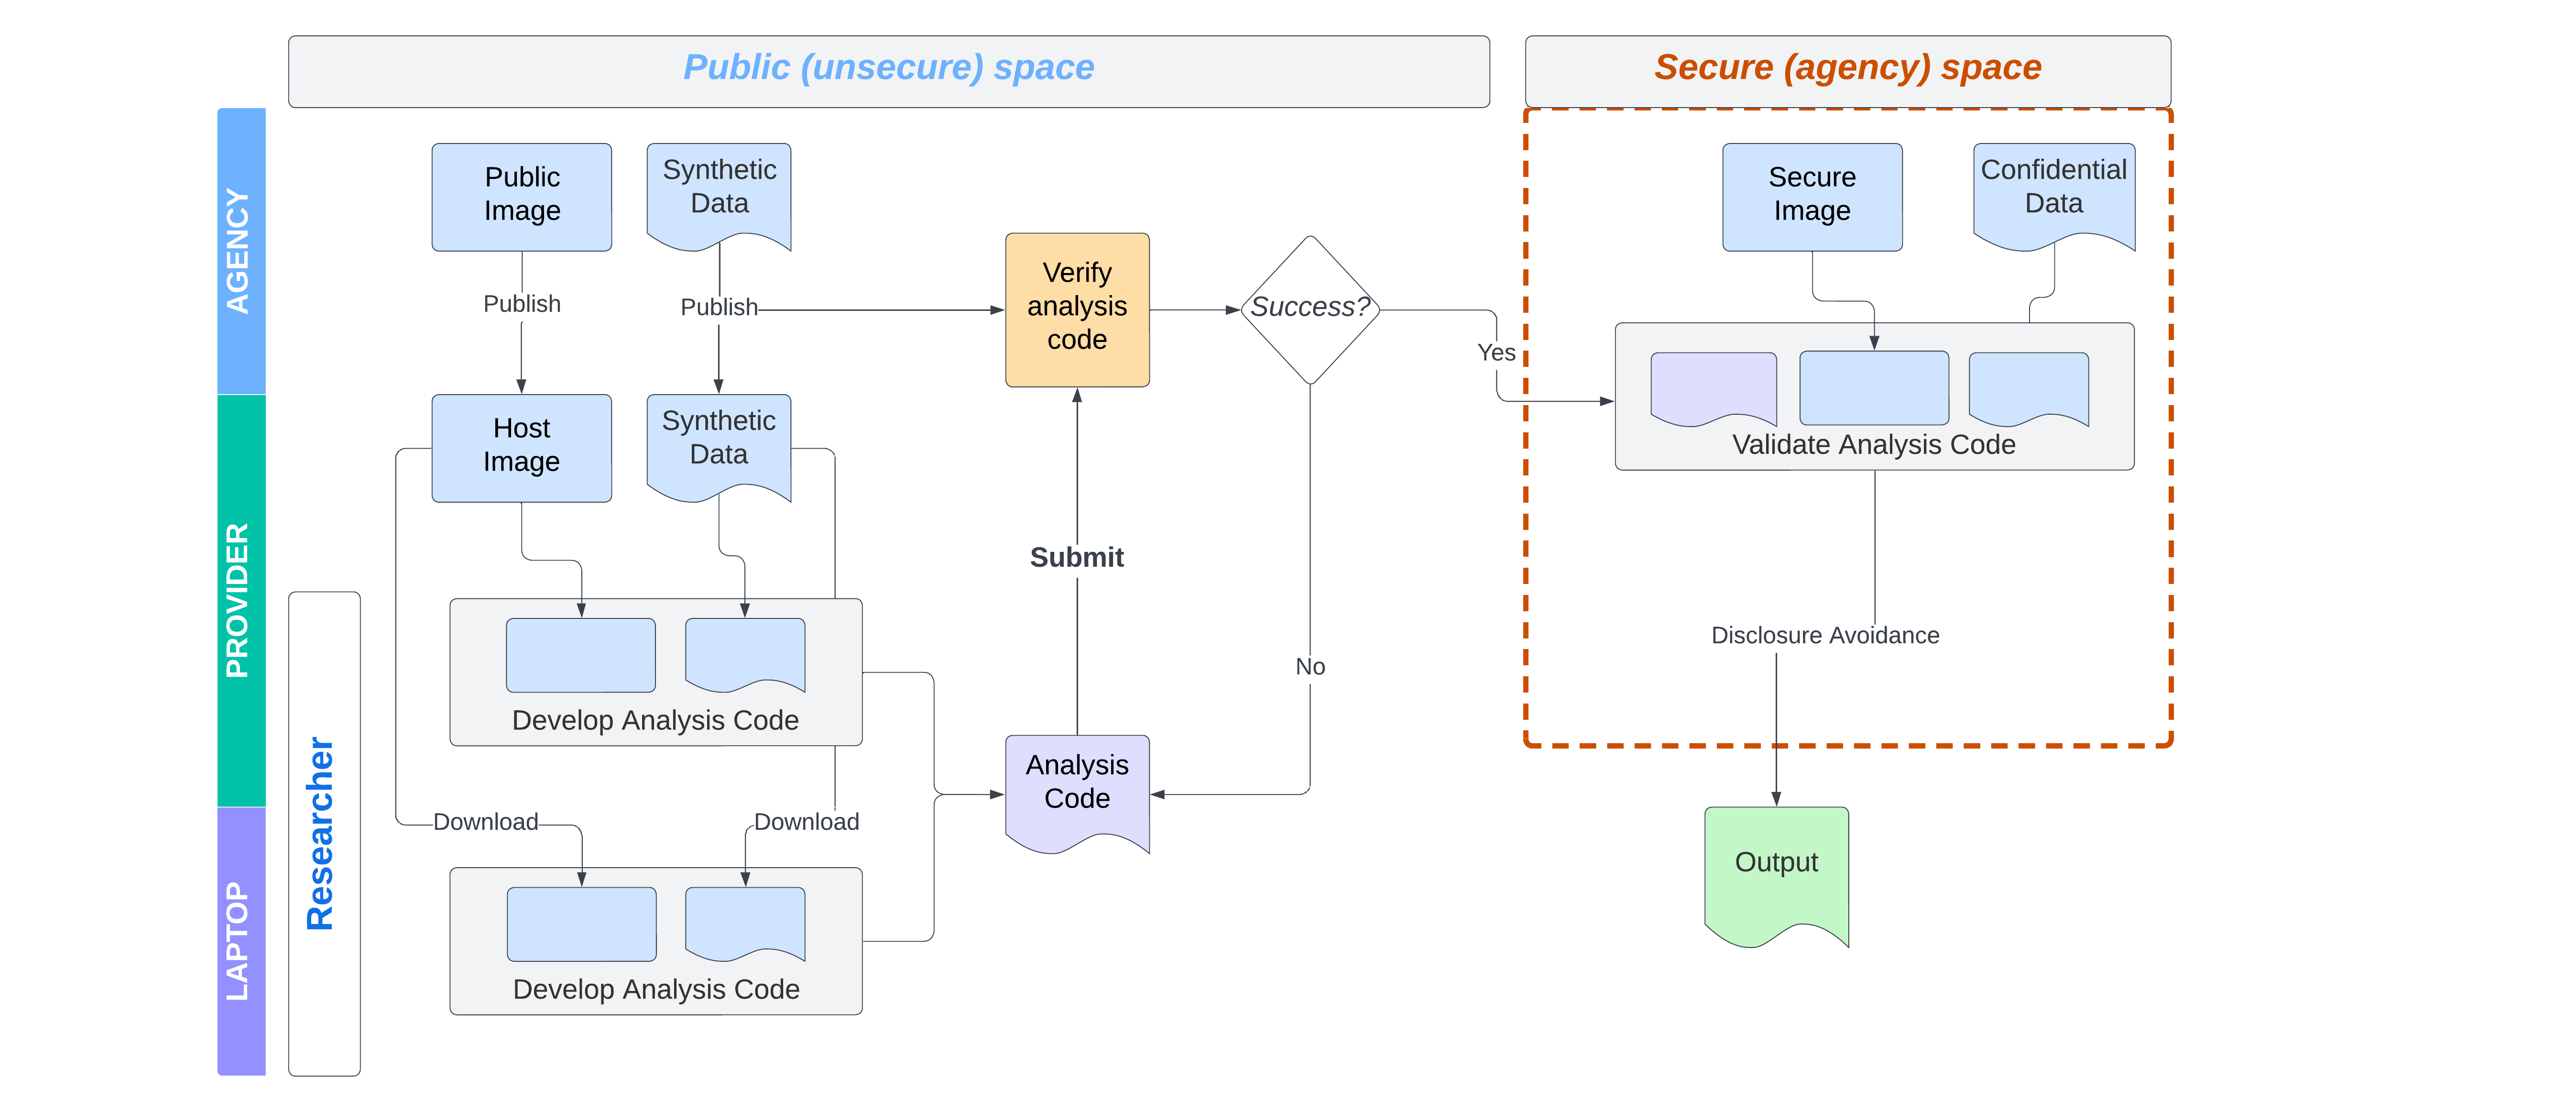
\includegraphics[width=1\linewidth]{NBER Docker Flow.png}
    % https://lucid.app/lucidchart/fe96a5a2-871b-468b-9bc3-b77fc6252b90/edit?viewport_loc=1150%2C-408%2C2735%2C1495%2Cm-5o7ONTd-nK&invitationId=inv_768c8ae5-f478-45d5-9886-068f7faf5d4b
    \caption{Sketch of a Docker-based workflow for validation of researcher code}
    \label{fig:docker-workflow}
\end{figure}

 Figure~\ref{fig:docker-workflow} provides a simplified process flow diagram, which can be compared to Figure~\ref{fig:ssb-flow}. Scalability of a system as described here hinges critically on having streamlined output vetting. Ideally, this  part must also be automated. At present, non-automation of output vetting is likely the single most important bottleneck of this system. However, the challenge of creating automated and reliable disclosure avoidance procedures is  not unique to the validation process described here.

\subsection{Other considerations, including additional security considerations}

For Stata (and/or R code), the security implications are no worse than those  faced by \ac{SSB} and SynLBD validation using the Cornell Synthetic Data Server, the current mechanism as of 2024 \citep{u.s.censusbureauSIPPSyntheticBeta2015b,us_census_bureau_validating_2023}, or in the present-day \ac{FSRDC}. They are similar to those faced by other systems, such as the German IAB \citep{bender_research-data-centre_2011,muller_institute_2021}. As noted above, it should be possible to do formal scans for malware and valid statistical code, and properly sand-boxed runs should allow for functional testing.

The example above uses \texttt{docker} as a container runtime. Docker is only one of the many container-running software environments. Some statistical agencies use \texttt{podman}. By its own documentation , \texttt{podman} is a full ``drop-in'' replacement for  \texttt{docker}, including the ``\texttt{build}'' functionality illustrated earlier in this document. \texttt{podman} does not require root privileges, one of the key concerns in general with \texttt{docker}. Apptainer \citep{noauthor_apptainer_nodate} is also an option, used for instance in the secure environment of the Bank of Portugal \citep{guimaraes_reproducibility_2023}, and is used in many academic high-performance computing environments. Data curators administrating a validation system should choose the one that is authorized within their IT environment. The basic principles illustrated above can be ported to any one of the alternate runtimes and image stores.

In principle, we would suggest running all of the various steps (initial check for reproducibility and security issues, final validation against confidential data) in a proper isolated and sandboxed environment. There is no reason the entire process needs to interact with the statistical agency's systems at large, up until the actual validation against the confidential data.

Statistical agencies should always rebuild the containers. Containers are layered (on other sites as well), allowing for the use of a properly security vetted container, running on a proper security vetted host. Some of the containers demonstrated within this document are built from a Codeocean image:

\begin{lstlisting}[language=docker]
FROM registry.codeocean.com/codeocean/stata:16.0-ubuntu18.04
\end{lstlisting}

\noindent but can just as easily be created from a base image maintained by one of the authors with full transparency:

\begin{lstlisting}[language=docker]
ARG SRCVERSION=17
ARG SRCTAG=2022-01-17
ARG SRCHUBID=dataeditors
FROM ${SRCHUBID}/stata${SRCVERSION}:${SRCTAG}
\end{lstlisting}

\noindent The use of a  (currently nonexistent) \textbf{public}  Census-sanctioned image might be used for the first step:

\begin{lstlisting}[language=docker]
FROM registry-public.census.gov/validation/stata:17.0-rh-secure-public
\end{lstlisting}

\noindent and would simply be replaced by an equivalent but fully security compliant internal image when rebuilding the image in the confidential environment:

\begin{lstlisting}[language=docker]
FROM registry.census.gov/validation/stata:17.0-rh-secure-internal
\end{lstlisting}



\subsection{Scalability}

For users to accept the restrictions of the synthetic data, it should scale better. So many of the vetting/building/running parts should (can easily) be streamlined. One key piece missing: standardized/streamlined output vetting.

\subsection{Data licensing}

One key condition for such a system is the ability to post synthetic data publicly, albeit  classified and published as ``experimental data.'' In contrast to the Cornell (or any other) Synthetic Data Server, the public component of the system would no longer have control over dissemination of the synthetic data files, but continue to have control over validation.\footnote{I do note that the European concept of a ``scientific use file'' does allow for controlled dissemination to certified educational institutions.}

As an added benefit, by compiling a library of container-based scientific uses of a particular dataset, the data provider can test out new data releases, alternative disclosure avoidance methods, or replacement data sources  at scale against prior scientific findings. This is currently not (easily) feasible - most such re-validations are painstakingly manual, and limited in scale, as noted earlier. The benefit would be improved user input on new and novel methods and data.


\section{Discussion}


% \begin{enumerate}
%     \item the mechanism must support arbitrary modeling approaches and ideally a large number of programming languages
%     \item the mechanism must allow for development of models by researchers that are close to their ``normal'' method of developing models
%     \item the mechanism must be low-cost for the data provider, scaling at best sub-linearly with the number of users of those datasets
%     \item the mechanism must be low-cost for the data user, imposing at best marginal costs on their existing research infrastructure (software, computers)
%     \item the privacy-protected data provided as part of such mechanisms must be good enough to allow for complex modeling
%     \item validation, if necessary, must be fast - on the order of hours
% \end{enumerate}

\subsection{Returning to the desiderata}

Containers satisfy most of the desiderata outlined earlier: 
\begin{enumerate*}[label={[D\arabic*]}, itemjoin={{; }}, itemjoin*={{, and }}]
    \item the Docker-based mechanism supports arbitrary modeling approaches, and in principle a large number of programming languages (modulo what the agency allows)
    \item the Docker-based mechanism  allows for development of models by researchers on their personal computer, if necessary, as long as they subsequently test their model within the prescribed Docker-based mechanism themselves
    \item the mechanism is low-cost (or even at no cost) for the data provider, and can be scaled up effectively; the costs are born by the compute providers (and possibly charged to the user)
    \item the mechanism can be low-cost for the data user: Most current cloud computing solutions that support this are at a trivial cost to the data user, and may be born by their institution (academic or otherwise). Alternatively, development on their own personal computer imposes no additional cost
    \item current privacy-protected data (SynLBD, SSB) are  good enough to allow for complex modeling, and the low-cost nature of the validation process allows for the development of additional synthetic data releases that trade off statistical accuracy for modeling utility, which is likely to be much simpler
    \item validation can be technically fast, albeit with a caveat.
\end{enumerate*}

\subsection{Some caveats}

Two caveats are in order. First, [D5] is contingent on finding an acceptable mechanism to rapidly generate useful synthetic data, possibly model-dependent. Tools for that exist \citep{synthpop,synthpop2016}, and the disclosure-avoidance analysis is improving \citep{SnokeEtAl2017}. However, in order for validation not just to be fast to process, but also fast to release to the user ([D6]), agencies need to accept and deploy privacy-protection mechanism that can scale. Current mechanisms in restricted-access data centers (FSRDC, \ac{CRDCN}, \ac{FDZ}) are often manual \citep{brandt_guidelines_2010}, albeit first attempts at using \acp{LLM} to speed up the process are being actively developed \citep{rigaud_checking_2023}.

\subsection{Addressing implementation issues}

While much of the technology is straightforward ``off-the-rack'' technology, the fact that it is not being used by statistical agencies or survey institutes suggests that some training is required and guidelines for deployment needed. 
%
\begin{enumerate*}[label={(\arabic*)}, itemjoin={{ }}]
\item Guidelines for agencies on how to prepare container specifications reflective of their internal execution environment, taking into account industry best practices on container specifications, security considerations, and usability are a necessity. NIST has some guidelines \citep{souppaya_application_2017}, and guidelines for secure use of containers for applications abound, and can be easily adapted to internal use at agencies. What is less available are guidelines on how to publish such containers for public consumption, these will likely need to be developed, possibly in conjunction with the target audience.

\item Users may need some guidance on general use of containers, and how to use containers in conjunction with this mechanism. There are many training documents and class notes available for general use of containers \citep{boettiger_introduction_2015,nust_automatically_2017,mcdermott_data_2023,the_turing_way_community_containers_2024,eyers_reproducible_2020,docker-stata,aea_data_editor_use_2021}, but few of them are actually known to most (academic) social scientists. How to use this specifically for the purpose of validation may need some training, though I suspect less so then the use of an idiosyncratic desktop platform that is even less familiar to users, as the \ac{SDS} was. Financial incentives might be used for a pilot phase.  
\end{enumerate*}

\subsection{How do we know it works?}
% metrics

The premise of my proposal is that it is easier and cheaper to implement. At present, the creation of highly protective synthetic data, and the supporting infrastructure for validation, is complex and therefore expensive.\footnote{The \ac{SDS} was supported by Sloan Foundation and \ac{NSF} grants as well as Census Bureau staff time over more than a decade, and the aforementioned project for synthetic IRS data is supported through grants by the Sloan Foundation, each of which was typically a multi-year project with cumulatively several million dollar support.} How would we know if this is cheaper? Implementing  agencies could track how much time was spent on submissions that were submitted with manual validation, how much time is spent managing complex data access protocols (when researchers themselves need to access the confidential data), and compare that to automated submissions under the current proposal (ideally in a randomized experiment),  allowing an assessment of the first-order impact on costs at the agency. Other cost factors might apply as well, for instance if the agency does not currently use containers, implementation costs of deploying software to manage submissions in such an automated way. IT personnel hopefully is aware of what it means to run containers within a large organization, but may need to adapt it to the particular research environment.  Non-pecuniary metrics might include the increase in usage of datasets, as well as in the number of validation requests. Second-order cost increases through expanded use remain hard to measure, and would need to be assessed in a broader cost-benefit analysis. Security and cost considerations might also affect the allowable set of software that can be used in containers, though it is an open question whether restricting users to specific software packages truly is an impediment to data use.\footnote{Observationally, the usage of SAS in the broader academic community in the social sciences is approximately zero, yet many replication packages that are associated with \ac{FSRDC} or \ac{CRDCN} projects still contain SAS code.}

\subsection{Possible extensions to more complex frameworks}

A critical bottleneck is disclosure avoidance, in part because the traditional analysis methods (both of public-use data and of synthetic data) are disclosure-avoidance agnostic, i.e., they do not incorporate prior or subsequent disclosure avoidance measures into the analysis method \citep{AbowdSchmutte_BPEA2015}. A first step is to include in the analysis container methods and metrics that allow users to assess how subsequent disclosure avoidance metrics will impact the releasable tables \citep{ReiterJPC2010}. For instance, prepared methods to apply traditional disclosure methods to the designated outputs \citep[aggregation, suppression, rounding, see][]{brandt_guidelines_2010} can be incorporated into the container. The \ac{SDS} already allowed to assess inference when combining estimates from multiple synthetic datasets (the \ac{SSB} provides four implicates). 

Applying methods that incorporate diffential privacy directly into the analysis methods \citep{alabi_hypothesis_2022,sheffet_differentially_2019,alabi_differentially_2023,chaudhuri_privacy-preserving_2008,alabi_differentially_2020} still provide incomplete coverage of the analysis methods used by social scientists \citep[see ][ for an overview]{barrientos_differentially_2021}. A promising but still preliminary system at this time is the IRS synthetic data file 
\citep{burman2018,tyagi_privacy-preserving_2024}. Whether such a system can be implemented with a simple container-based approach as outlined here remains to be seen. 

\section{In conclusion}

The use of containers for validation of analyses that were prepared using synthetic data ensures reproducibility, reliable portability, and enables scalability. The use of cloud-based commercial or university-based services requires no infrastructure or software maintenance by either data provider or users, and often no direct cost.  With very little effort, automation is possible (potentially through web forms), and the only likely  If   privacy-protection mechanisms can be tuned to acceptable protection levels (on par with traditional mechanisms that are applied to unrestricted public-use products), then validation can be made highly automated, and the quality of the synthetic data itself can be decreased, while maintaining high levels of user acceptance due to a fast validation process.






















\section*{Disclosure Statement}
The author has no conflicts of interest to declare. The mention of commercial entities is not meant to endorse any such providers, and the author holds no financial interest in any of the mentioned commercial entities.

\section*{Acknowledgments}

I have benefited from discussions with many folks, including Gary Benedetto, John Abowd, Rob Sienkiewicz, and from feedback following presentations to the National Academies, Census Bureau, and at the NBER conference on ``Data Privacy Protection and the Conduct of Applied Research.'' The original development of the idea was partially funded by \href{https://sloan.org/grant-detail/6845}{Alfred P. Sloan Foundation Grant G-2015-13903}.

\section*{Contributions}

LV conceived the topic, wrote the text, and prepared the examples. The statistical code used within the container, serving as a stand-in for any statistical analysis, was provided by Evan Totty, U.S. Census Bureau.  


%Begin appendix section(s)
\appendix

% Add appendices here:
%\section{Title}
%\label{appendix-customize-this-label}
%Lorem ipsum dolor sit amet, consectetur adipiscing elit. Pellentesque id massa vulputate, tristique mi id, imperdiet mi. Mauris id ante ac lacus mollis sagittis. Sed imperdiet nibh id eros malesuada, at fermentum urna mollis. Sed id elit eu arcu varius tempor tincidunt in orci. 



% All references should be stored in the file ``references.bib``
% Please do not modify anything below this line.
\printbibliography

\newpage
\section*{Responses}

\begin{itemize}

\item Idea is akin to holdout samples (in computer science, but also social sciences \citep{liu_successes_2019}) 
\item "common task framework": research design from machine learning called the common task method \citep{donoho_50_2017,liberman_obituary_2010}. The common task method involves three main elements: a common target for predictive modeling, a common error metric, and a common data set with both training data available to participants and held-out data used for evaluation. \citep{liu_successes_2019}

\end{itemize}

\textbf{General responses}

\begin{response}
    Thank you to the editor and the reviewers for their valuable input, which I very much appreciated, and which I believe has lead to substantial improvement of the text. I have revised the structure of the text, and linked it with various other efforts highlighted by the reviewers. 

    \begin{itemize}
        \item I have added a new introduction that lays out what the article intends to convey, and what tools it will describe. This should help make it clearer from the start, and should have been included; my apologies for only adding it now.
        \item I then follow with a section that describes and situates the various concepts, both those that might be new to some in the readership (``containers'') and those that might be known, but possibly ambiguously defined and used in a broader context (first among them: ``synthetic data''). This was a request by multiple reviewers, suggesting that it is still a necessary structure to provide. I will note that I had previously talked with others in the open (social) science field, who very much implied that even the late definition of containers was ``very pedantic'' because apparently everybody (should) know about that by now... highlighting the wide diversity in information dispersal even within the narrow "field" of social science. I hope that the current definitions strike a good balance.
        \item I have also replaced Figure 1 with a better figure, referenced it in the text, and added Figure 5, which shows the equivalent process flow for the Docker-based approach.
    \end{itemize}
\end{response}

%\subsection*{To editor}
\textbf{To editor} 

\begin{referee}
As you can see from the three reports attached,
the reviewers are generally positive about the topic, but have a number of non-trivial concerns and
suggestions on the substance (especially from Reviewer 1) and on the paper organization and
presentation. Reading it myself I can see why Reviewers 2 and 3 find it difficult to see quickly what the
article is about. I surmise the concept of "container" is not a commonly understood one, and even
after I read its description in Section 5, it is not immediately intuitive why it can protect data privacy at
scale. Of course that reflects my ignorance, and your article is to educate people like me. Although I
am of sample size 1, I'm quite confident that over 50\% of statisticians are as clueless as I am on this
topic. :-)
For people like me, the article would be much more enticing if it starts with defining the container,
and explain it intuitively in what ways it helps to protect data privacy, and can do so at scale. Then
you can discuss why other methods are inferior and in what way. 
\end{referee}

\begin{response}
    I have now added a new introduction that lays out the goal of the article, and then added/reformated a section on concepts and prior science, which should hopefully address this point.
\end{response}

\begin{referee}
By the way, the list of desiderata in
Section 6 is great,
but I am a strong believer of the no-free lunch principle. I'd be very happy to be wrong here, but
suspect in many practical situations, one may need to prioritize some. If so, some discussions on how
to prioritize may make readers pay more attention to the list, as those who find the list too
demanding or idealistic might choose to ignore it.

\end{referee}

\begin{response}
    I address this in an expanded conclusion.

    \vspace{1em} I have also linked the various code fragments more closely to the text, explaining in more detail what they do, for those not necessarily familiar with the code. I have also corrected a few inaccuracies not noted by the referees when describing the setup of the container in the example.
\end{response}


\textbf{Reviewer 1:}

\begin{referee}
    
The manuscript centers on the use of container technology to improve access to confidential data for research while ensuring data privacy and security.  The manuscript outlines how containers, in combination with synthetic data and controlled environments like Codeocean, provide researchers and data stewards with a compatible setup that facilitates statistical analysis on confidential datasets while preserving privacy.  The manuscript discusses how containers create reproducible, secure environments that can be deployed on public or private infrastructure, enabling researchers to develop and validate code on synthetic data.  Once validated, this code can be securely transferred to confidential environments for final analysis.  The manuscript emphasizes the scalability, reproducibility, and importance of disclosure avoidance procedures enabled by containers, ensuring sensitive information remains protected throughout the research process.  It also acknowledges that, although the use of containers helps mitigate scalability issues, a major bottleneck in scaling this system will still lie in the need for automated output vetting, which remains a key challenge in disclosure avoidance.
\end{referee}

\begin{response}
    Thank you for the succinct summary, which is better than mine! I have expanded the intro, and included a summary which I hope is as inteligible as yours.
\end{response}

\begin{referee}

The manuscript presents a strong case for using containers to improve access to confidential datasets while preserving privacy.  By using containerization, the approach enhances reproducibility through a standardized environment as researchers can conduct analyses within consistent configurations.  This setup enables data stewards to establish clear boundaries, such as specific software versions and dependencies, which helps ensure a controlled and reproducible workflow.  Managing these parameters creates an environment where analyses can be reliably repeated or validated. The approach aligns well with best practices in secure data handling. The requirement for researchers to provide only their code, combined with the container's capacity to be rebuilt within a secure environment, adds efficiency to the process.  An implementation of this idea by an institution committed to providing access to confidential datasets while safeguarding privacy would be valuable.  


\end{referee}

\begin{response}
    Thank you for that. I hope you are also the reviewer for our grant application.
\end{response}

\begin{referee}

Below are some suggestions to further strengthen the manuscript.

A valuable addition to the manuscript would be a subsection (or adding some paragraphs) discussing metrics that institutions might consider when evaluating the feasibility of container-based secure environments for accessing and analyzing confidential datasets.  Some potential metrics could be:
    \begin{itemize}
        \item Hardware and infrastructure costs associated with supporting container technology, especially if large datasets or complex analyses require substantial computational resources. 
        \item Number of validations that can be completed in a given period of time, such as per week. 
        \item IT personnel costs, as institutions will likely need staff skilled in containerization, data security, and privacy protocols to set up and maintain these environments effectively. 
        \item Learning costs for both internal and external users, including the time and resources required to train users unfamiliar with container technology. 
        \item The types of software, programming languages, and analysis tools that potential users currently rely on.  This information, possibly gathered through a user survey, can guide institutions in configuring containers with compatible software and dependencies. However, institutions may face challenges in surveying a representative sample of potential users. 
    \end{itemize}

\end{referee}

\begin{response}
    Thank you for that suggestion. We did actually include the first two of those metrics in our grant application, and \textbf{I have expanded what was previously called a Conclusion} (somewhat presumptively), which is now \textbf{Discussion}, discussing the desiderata (as requested by the Editor) and these metrics. While I don't (here) expound on the survey for required tools, I do mention that institutions should be aware of the tools being used in the community that they serve, for instance by looking at the distribution of software used in replication packages. 
\end{response}

\begin{referee}

    Compliance with relevant laws.

\end{referee}

\begin{response}
    I did not address this issue explicitly, because I assumed that no laws need to be changed in order to implement this mechanism. I did add a footnote, identifying this assumption, when discussing disclosure avoidance.


    \begin{quote}
        Footnote: I call this ``usual'', since I make no assumptions about changes to existing laws on data confidentiality that an agency is subject to. In order to be implementable, all data access, whether directly or via this new mechanism, must still be compliant with the laws that the agency is subject to, though some re-interpretation of what are permissible uses may be a separate channel to speed up access.
        \end{quote}
\end{response}

\begin{referee}

    The code snippets provided in the document are a valuable addition, moving the discussion from theory to application and giving readers actionable steps to set up their containerized environments.  This hands-on approach makes the concept more accessible, especially for those looking to replicate or test the methods described.  To further enhance clarity, it would be beneficial to include more inline comments within the code snippets to explain relevant lines, particularly for readers unfamiliar with Dockerfile syntax and Stata commands. 
\end{referee}

\begin{response}
    This is a good point, though I subject this to the Editor's filter of how long an article should be. I now explicitly link to the Github repository with the complete example, and have added comments there, as a hopefully acceptable compromise.
\end{response}

\begin{referee}


    The distinction between "reproducible run" and "validating researcher-provided code" in Sections 6.3.2 and 6.3.4 could benefit from further clarification, as these terms may seem similar yet serve distinct purposes.  In Section 6.3.2, the term "reproducible run" appears to refer to an initial execution of code on CodeOcean's infrastructure to confirm that the code runs without technical errors though this does not guarantee that all necessary code has been executed, as sections of code may be commented out or non-functional.  In contrast, Section 6.3.4 describes a "validation" step where the replicator, or data custodian, re-runs the container on synthetic data to ensure reproducibility in a non-secure environment if there are any doubts or if initial validation wasn't completed on CodeOcean.  While someone with a computer science background might quickly understand these nuances, broader audiences might find the distinction confusing. For this reason, it would be beneficial for the manuscript to elaborate on these two steps, clarifying their distinct roles in the reproducibility and validation process. 
\end{referee}

\begin{response}
    This is a good point, though I subject this to the Editor's filter of how long an article should be. I now explicitly link to the Github repository with the complete example, and have added comments there, as a hopefully acceptable compromise.
\end{response}

\begin{referee}

    The document could benefit from addressing ongoing developments in the use of validation servers, particularly those leveraging differential privacy to automate output vetting.  Several research organizations are exploring validation servers because they allow institutions to control how users submit queries and specify the types of output that can be released, facilitating integration with differential privacy.  Implementing a similar approach with containers raises interesting possibilities and potential challenges. For example, it could be feasible to set up containers equipped with OpenDP, enabling users to run analyses with differential privacy settings on synthetic data.  This setup could allow users to test analyses within a "reasonable" privacy budget and compare the outputs against those obtained using standard statistical software that does not employ differential privacy. However, with the proposed approach based on container technologies, there are likely to be significant challenges in automating output vetting through differential privacy within a secure environment. The manuscript should address these challenges if they exist.  Additionally, requiring users to conduct their analyses in OpenDP may introduce a steep learning curve. 
\end{referee}

\begin{response}
    TBD
\end{response}

\begin{referee}


    In a similar vein, instead of choosing between validation servers and containers, there could be potential in integrating these technologies.  For instance, validation servers could be \textit{containerized and distributed across institutions}, allowing researchers to submit queries locally.  These queries could then be routed to a centralized secure environment, such as one maintained by the Census Bureau, ensuring controlled and consistent query processing across institutions.
    Including a discussion of these ideas in the document's discussion section would provide valuable insight into how containers and validation servers could work together to advance secure, scalable access to confidential data, and automatic output vetting.
\end{referee}

\begin{response}
    The suggestion is intriguing, but highlights issues of trust and certification between institutions - not insurmountable, but also probably not lightweight (as we have investigated in a separate project \url{https://transparency-certified.github.io/} that has not yet written up the ideas).

    For now, I have simply added universities in the discussion:

    \begin{quote}
        Providing evidence of successful reproducibility (validation) may require the use of third parties, such as aforementioned commercial providers, but also universities or other research institutions. 
    \end{quote}
\end{response}

\begin{referee}

     There are several minor comments that need to be addressed in the manuscript:
    \begin{itemize}
        \item Ensure all typos are corrected (like Howver) and that all acronyms and initialisms are clearly defined upon first use (like SSB, FSRDC). 
        \item There is no reference to Figure 1 in the main text. If possible, the provided diagram in Figure 1 could include information on where containers are used or rebuilt to clarify the workflow. 
        \item On page 11, the purpose of the sentence, "which runs for about 3 minutes on a 2021-vintage Linux workstation," is unclear.  Consider clarifying its relevance to the reader. 
        \item On page 9, the phrase "(need cite)" appears and should be replaced with an appropriate reference. 
         \item In section 6.3.4, the sentence, "Should the data custodian have doubts about the verified run of the capsule," requires further clarification on why the data custodian might have doubts about the capsule's verified run. 
    \end{itemize}

\end{referee}

\begin{response}
    Response begins here.
\end{response}

\textbf{Reviewer 2:}

\begin{referee}
    Solutions to issues in both researcher access to confidential data and reproducibility of
results are important, and this paper addresses these issues in novel ways and demonstrates very
compelling applications at a federal agency. Even reading the paper carefully it was difficult to discern
the main conclusion and contribution from the various discussions though. Renaming the manuscript
to relate to Census data, or the facilitation of research on synthetic data, might help the reader since
the current title implies a new innovation in HIPAA compliant containers. Nonetheless there should be
a discussion about the relationship of this contribution to the costs of requirements to obtain HIPAA
compliant containers vs relying on synthetic datasets. 
\end{referee}

\begin{response}
    I appreciate the viewpoint, as I had been blissfully ignorant of HIPAA  compliant containers - these are simply not present in any of the discussions in the social science data confidentiality setup that I have been involved in. In economics as much as in sociology and political science, most academics do not even know what containers are, and certainly don't interact with HIPAA in almost any circumstance.

    I have reviewed what one can learn about HIPAA compliant containers, the context in which they are deployed, and identify where there is a connection. As the reviewer managed to glean from my previous version, the context here is not in securing containers, but in using unsecured containers - those that do not need to be secured - to improve access. I reference a few situations - not just HIPAA - where containers are used in secured environments. Most of those that I am aware of are deployed within an entire environment that is secure by whatever rule (not HIPAA, but GDPR or US Government security), and so the internal structure is less important. I hope this properly delineates the current approach from others where containers themselves play a more dominant role.
\end{response}

\begin{referee}
    
After I realized the manuscript was not on
technical developments for containers, I got the impression it was a discussion of human interaction
with a pilot design for an experiment at the Census bureau, but the manuscript
does not take this further. In short the manuscript needs rewriting for improved clarity at the outset,
including clearing stating the purpose of the work, what the work was, and the findings.

\end{referee}

\begin{response}
    I hope that the present rewrite clarifies this, with changes throughout the text.
\end{response}

\begin{referee}
    
There is
related work in applications of the "Common Task Framework" (see Donoho 2024 \url{https://doi.org/10.1162/99608f92.b91339ef})
and using a container as a reproducible pipeline for checking against withheld test data by a federal
agency (e.g. NIST) should be compared to the approach presented here. 

\end{referee}

\begin{response}
    I now relate to the Common Task Framework, but delineate from the challenge paradigm that Donoho (2024) and others reference. In Donoho's classification, this is meant (possibly) for exploratory analysis. 
\end{response}

\begin{referee}

The authors also appear to
be presenting new standards for reproducible research code publication (e.g. section 6.1) yet don't
reference the extensive body of literature on this topic. 

\end{referee}

\begin{response}
    This was absolutely not meant as a new standard for research code publication. There are too many standards already (none of which is followed in the social science literature that I am familiar with). This is meant purely as a requirement of the validation. I have clarified that.
\end{response}

\begin{referee}
    
Ideally a link to their census example can be
included in the manuscript, allowing readers to try out the example. 

\end{referee}

\begin{response}
    I have added a link to the Github repository for the example.
\end{response}


\begin{referee}
The ideas in the manuscript will
generate lots of reader interest if they can be presented more clearly.
\end{referee}

\begin{response}
    Thank you for your feedback!
\end{response}


\textbf{Referee 3}

\begin{referee}
    A definition of containers should be included in the abstract. 
\end{referee}

\begin{response}
    TBD
\end{response}


\begin{referee}
  It should also be included
early in the main body of the text. \end{referee}

\begin{response}
   Excellent point, and I have added it there.
\end{response}


\begin{referee}
At the very least, the author should consider including a short
roadmap paragraph at the beginning of the paper so that readers know what to expect. Right now, as
is written, containers do not appear until Section 5, leaving readers wonder what the paper is really
about before reaching that point.
\end{referee}

\begin{response}
    You are absolutely right, and this has been (hopefully) corrected.
\end{response}


\begin{referee}

2.
The Media Summary seems missing.

\end{referee}

\begin{response}
    TBD
\end{response}


\begin{referee}

3.
Section 2 paragraph 1: SSB is not defined nearby, but rather in Section 6.

\end{referee}

\begin{response}
    Apologies for that oversight.
\end{response}


\begin{referee}
4.
Table 1: It is unclear what each column is about until reading relevant text. It would be helpful to
add some information about the confidence interval overlap, such as "the closer it is to 1 the higher
the utility" in the table caption.
\end{referee}

\begin{response}
    Apologies for that oversight.
\end{response}


\begin{referee}
5.
Figure 1: It is not mentioned in text what Figure 1 is for and about.

\end{referee}

\begin{response}
    The figure was aspirational. I have simplified the figure, and juxtaposed it to the proposed workflow, which hopefully provides additional clarity.
\end{response}


\begin{referee}
6.
Page 5 middle paragraph: The second sentence starts with talking about Statistic Canada and
microdata.no but ends with the 2018 paper.

\end{referee}

\begin{response}
    I'm not sure what this comment refers to. All four examples refer to examples of scaling up access to restricted-access data, and are discussed (very briefly) in the next sentence. (``scale up access to
confidential data. To cite a few examples,...'' No change was made.
\end{response}


\begin{referee}

7.
Page 5 last paragraph: The author talks about "social sciences" generically but the reference is
on economics. Some edits should be added.

\end{referee}

\begin{response}
    Thank you for pointing that out. The reference is to economics replication packages, since that provides a measurable statistic. I am not aware of a similar collection effort for sociology or psychology, possibly in part because it is harder to parse each article's reproducible materials at scale. I have added this explanation in a footnote, 

    \begin{quote}
        Footnote: Code run in November 2023, searching for any filename that contained the strings `main' or `master', the most common name used for control code in economics. I am not aware of a similarly comprehensive collection for other social sciences. 
        
        \vspace{0.5em} \noindent Text: This is also my impression from our own efforts at the LDI Replication Lab supporting the AEA Data and Code Availability Policy, though we no longer make a systematic effort to categorize this. 
    \end{quote}
    
    
and expanded the reference to point to the various metastudies documenting reproducibility challenges in sociology, economics, political science, and psychology. 

    \begin{quote}
        Footnote: I define ``interactive computing'' as any sequence of computational codes that must be explicitly --- through edits --- adapted to the environment it is running in, and/or does not have a streamlined workflow that can be triggered from a single file, regardless of workflow technology. Examples of workflow management ``systems'' range from \texttt{make} (1976) \citep{association_for_computing_machinery_acm_2003} to \texttt{Snakemake} \citep{molder_sustainable_2021}, to literate programming tools such as \texttt{Sweave} \citep{Leisch2002SweaveDG} and Quarto \citep{Allaire_Quarto_2024}, to simple concatenated calls to software (canonical \texttt{run.sh}). 
        
        \vspace{0.5em} \noindent Text: Examples abound, and can often be gleaned from the fact that many of the reproducibility meta-studies only succeed in reproducing a small number of studies due to limitations in personnel time.

        \vspace{0.5em} \noindent Footnote: \citet{stockemer_data_2018} note ``lack of organization in code and data presentation was the main reason that we were unable to replicate some results'' in political science articles. \citet{StoddenPNAS2018} notes that only 32\% of packages in Science required only minor or no effort to reproduce, though some of the reasons listed are unavoidable (GPU setup, custom hardware) and not related to workflow issues. For the economics journal studied in \citet{herbert_reproduce_2024}, only 24\% required no change to the code in order to be able to run, even when the ultimate results was full reproducibility.
    \end{quote}


\end{response}


\begin{referee}
8.
Section 6.2: The first sentence seems incomplete.

\end{referee}

\begin{response}
I'm not sure I follow, though I think the sentence is maybe too long. The sentence in the submitted version, this sentence read 
    \begin{quote}
6.2. \textbf{Validating reproducibility}. In its base configuration, Codeocean signals to researchers the
successful completion of a run of the controller script ‘run‘ in the right pane of the user interface,
indicating to the custodian of the confidential data that the code is verified to execute on the
synthetic data.
\end{quote}

I have rewritten this to be grammatically somewhat less complex, but also maybe clearer in what I wanted to convey.

\begin{quote}
    The Codeocean interface signals to researchers the successful completion  of the controller script (called \texttt{run}) in the right pane of the user interface. To the custodian of the confidential data, this indicates that the code is verified to execute without error on the synthetic data. The results produced by this specific run of the controller script, and not any previous interactive run, are the results provided in the ``results'' pane. This is important for scalability and efficiency, as it reduces the need for extensive debugging, on the researcher side, and allows for rapid assessment of basic reproducibility by the data custodian.
\end{quote}

\end{response}


\begin{referee}

9.
Any comments/references/examples with Python?

\end{referee}

\begin{response}
    The example is provided as Stata, because most of the users in economics (the original addressees) are Stata users. However, I now point out that this is purely for illustrative purposes. If desired by the reviewer and editor, an equivalent R example could be constructed as a supplement to the existing Stata-based Github example. A python example would not be useful for social scientists, given the low user base there.
\end{response}

\end{document}
